%% arara directives
% arara: xelatex
% arara: bibtex
% arara: xelatex
% arara: xelatex

%\documentclass{article} % One-column default
\documentclass[twocolumn, switch]{article} % Method A for two-column formatting

\usepackage{preprint}

\usepackage{enotez}
\let\footnote=\endnote

%% Math packages
%\usepackage{amsmath, amsthm, amssymb, amsfonts}

%% Bibliography options
%\usepackage[numbers,square]{natbib}
%\bibliographystyle{unsrtnat}
\usepackage{natbib}
%\bibliographystyle{Geology}

%% General packages
\usepackage[utf8]{inputenc}	% allow utf-8 input
\usepackage[T1]{fontenc}	% use 8-bit T1 fonts
\usepackage{xcolor}		% colors for hyperlinks
\usepackage[colorlinks = true,
            linkcolor = purple,
            urlcolor  = blue,
            citecolor = black,
            anchorcolor = black]{hyperref}	% Color links to references, figures, etc.
\usepackage{booktabs} 		% professional-quality tables
\usepackage{nicefrac}		% compact symbols for 1/2, etc.
%\usepackage{microtype}		% microtypography
%\usepackage{lineno}		% Line numbers
\usepackage{float}			% Allows for figures within multicol
\usepackage{textcomp,marvosym}
%\usepackage{multicol}		% Multiple columns (Method B)

%\usepackage{lipsum}		%  Filler text
\usepackage{lettrine}
\usepackage{pdflscape}
\usepackage{longtable}
\usepackage{threeparttablex}

 %% Special figure caption options
\usepackage{newfloat}
\DeclareFloatingEnvironment[name={Supplementary Figure}]{suppfigure}
\usepackage{sidecap}
\sidecaptionvpos{figure}{c}

% Section title spacing  options
\usepackage{titlesec}
\titlespacing\section{0pt}{12pt plus 3pt minus 3pt}{1pt plus 1pt minus 1pt}
\titlespacing\subsection{0pt}{10pt plus 3pt minus 3pt}{1pt plus 1pt minus 1pt}
\titlespacing\subsubsection{0pt}{8pt plus 3pt minus 3pt}{1pt plus 1pt minus 1pt}


%%%%%%%%%%%%%%%%   Title   %%%%%%%%%%%%%%%%
\title{The Precambrian paleogeography of Laurentia}

% Add watermark with submission status
%\usepackage{xwatermark}
%% Left watermark
%\newwatermark[firstpage,color=gray!60,angle=90,scale=0.32, xpos=-4.05in,ypos=0]{\href{https://doi.org/}{\color{gray}{Publication doi}}}
%% Right watermark
%\newwatermark[firstpage,color=gray!60,angle=90,scale=0.32, xpos=3.9in,ypos=0]{\href{https://doi.org/}{\color{gray}{Preprint doi}}}
% Bottom watermark
%\newwatermark[firstpage,color=gray!90,angle=0,scale=0.28, xpos=0in,ypos=-5in]{*correspondence: \texttt{swanson-hysell@berkeley.edu}}

%%%%%%%%%%%%%%%  Author list  %%%%%%%%%%%%%%%
\usepackage{authblk}
\renewcommand*{\Authfont}{\bfseries}
\author[]{Nicholas L. Swanson-Hysell}
\affil[]{Department of Earth and Planetary Science, University of California, Berkeley, CA 94720 USA}

\setcounter{section}{4}

%%%%%%%%%%%%%%    Front matter    %%%%%%%%%%%%%%
\begin{document}

\twocolumn[ % Method A for two-column formatting
  \begin{@twocolumnfalse} % Method A for two-column formatting
  
\maketitle

\begin{abstract}
Laurentia is the craton that forms the Precambrian core of North America and was a major continent throughout the majority of the Proterozoic following its amalgamation 1.8 billion years ago. The paleogeographic position of Laurentia is key to the development of reconstructions of Proterozoic paleogeography including the Paleoproterozoic to Mesoproterozoic supercontinent Nuna and latest Mesoproterozoic to Neoproterozoic supercontinent Rodinia. There is a rich record of Precambrian paleomagnetic poles from Laurentia, as well as an extensive and well-documented geologic history of tectonism. These geologic and paleomagnetic records are increasingly better constrained geochronologically and are both key to evaluating and developing paleogeographic models. These data from Laurentia provide strong-support for mobile lid plate tectonic processes operating continuously over the past 2.2 billion years. 
\end{abstract}
%\keywords{First keyword \and Second keyword \and More} % (optional)
\textit{This manuscript is a preprint of the chapter: \vspace{0.1 cm} \\
Swanson-Hysell, N. L. (2021) The Precambrian paleogeography of Laurentia. In: Pesonen, L.J., Salminen, J., Evans, D.A.D., Elming, S.-Å., Veikkolainen, T. (eds.) Ancient Supercontinents and the Paleogeography of the Earth.}
\vspace{0.3 cm}
  \end{@twocolumnfalse} % Method A for two-column formatting
] % Method A for two-column formatting

%\begin{multicols}{2} % Method B for two-column formatting (doesn't play well with line numbers), comment out if using method A


%%%%%%%%%%%%%%%  Main text   %%%%%%%%%%%%%%%
% \linenumbers

\subsection{Introduction and broad tectonic history}
\lettrine[lines=2]{L}{aurentia} refers to the craton that forms the Precambrian interior of North America and Greenland (Fig. \ref{fig:Laurentia_map}). Laurentia comprises multiple Archean provinces that had unique histories prior to their amalgamation in the Paleoproterozoic (ca. 1.8 billion years ago; Ga), as well as regions of Paleoproterozoic and Mesoproterozoic crustal growth that post-date this assembly (Fig. \ref{fig:Laurentia_map}; \citealp{Hoffman1989c, Whitmeyer2007a}). That the vast majority of the present-day continent of North America is a single Precambrian craton without major differential motion between constituent provinces and relatively minor crustal growth over the past billion years is exceptional in comparison to Earth's other continents. In contrast, South America and Africa are products of the amalgamation of multiple Proterozoic cratons that obtained their relative positions during the formation of Gondwana ca. 0.6 Ga \citep{Goscombe2019a}. Eurasia's constituent Proterozoic cratons have an even more recent history of amalgmation with the North China and South China cratons not arriving in their present relative position until ca. 0.15 Ga \citep{Van-der-Voo2015a,Torsvik2017a}. The longevity of a large intact Laurentia makes its position a critical part of global paleogeographic models since its assembly. Rich geologic, paleomagnetic, and geochronologic data provide deep insight into Laurentia's tectonic history and paleogeographic journey that is the focus of this chapter.

\begin{figure*}
\centering
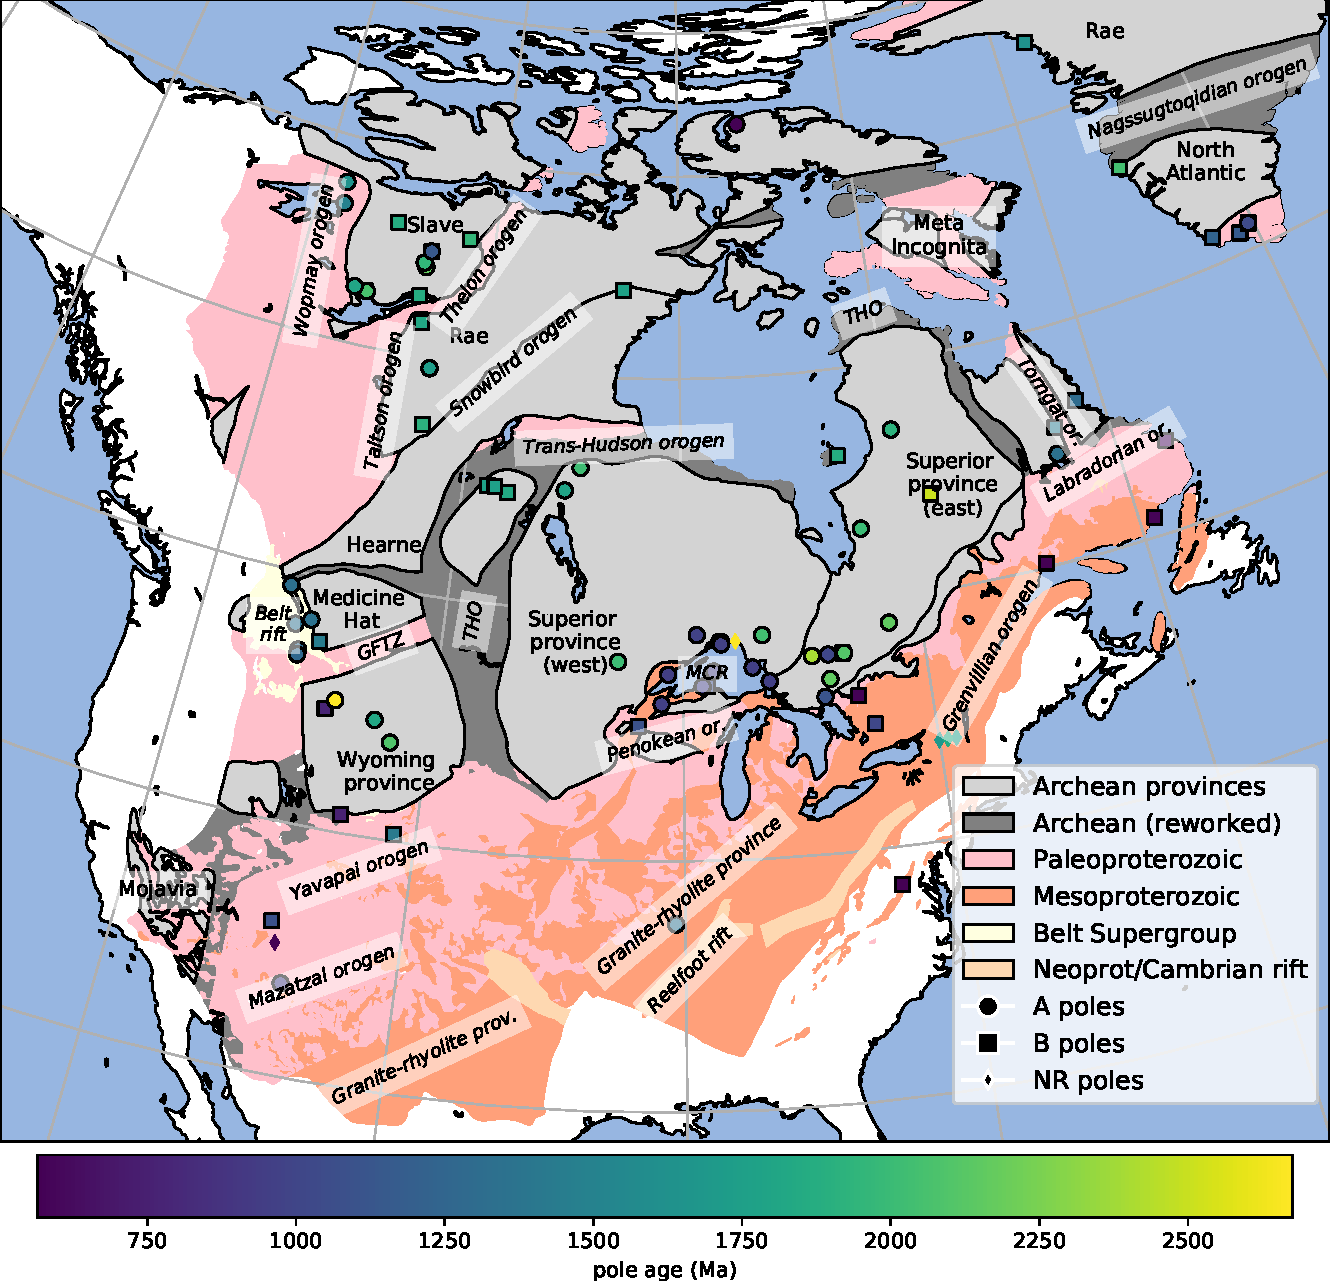
\includegraphics[width=\textwidth]{../Figures/Fig1_map.pdf}
\caption{\textbf{Simplified map of the tectonic units of Laurentia.} The Archean provinces (labeled with text) and younger Paleoproterozoic and Mesoproterozoic crust are simplified from \cite{Whitmeyer2007a} with additions for Greenland based on \cite{St-Onge2009a}. Proterozoic orogens are labeled with \textit{italicized text} (or. -- orogen; THO  -- Trans-Hudson orogen; MCR -- Midcontinent Rift). The localities from which the compiled Precambrian paleomagnetic poles were developed are shown and colored by age. The circles (A rated poles) and squares (B rated poles) have been assessed by the Nordic workshop panel \citep{Evans2021a} while the diamond (not rated -- NR) poles are discussed in the text.}
\label{fig:Laurentia_map}
\end{figure*}

\subsubsection{Laurentia's initial formation}
Collision between the Superior province and the composite Slave\endnote{The term Slave Province is rather jarring when read for the first time given that it brings to mind evil human oppression. The geologic Slave Province as well as the eponymous Great Slave Lake get their name from a name given to the First Nation indigenous peoples of the Dene Group who are indigenous to the region. The origin of the name Slave is commonly explained as a French translation of the name given to the Dene people by the Cree people \citep{Britannica-Slave2017a}. Given its negative connotations, the name is not preferred now and there are efforts to remove it from Canadian place names \citep{Mandeville2016a}. Given that this name for the Archean geologic province is deeply entrenched in the geologic literature it will be used here.}+Rae+Hearne provinces that resulted in the Trans-Hudson orogeny represents a major event in the formation of Laurentia (Fig. \ref{fig:Laurentia_map}; \citealp{Corrigan2009a}). Terminal collision recorded in the Trans-Hudson orogen is estimated to have occurred ca. 1.86 to 1.82 Ga based on constraints such as U-Pb dates of monazite grains and zircon rims \citep{Skipton2016a, Weller2017a}. It was preceded by a period of accretionary and collisional orogenesis that is recorded in the constituent provinces and terranes of Laurentia leading up to the terminal collision of the Trans-Hudson orogeny. Throughout this chapter, I will utilize the term ``accretionary orogenesis'' in a broad sense to refer to the tectonic addition of allochthonous terranes such as island arcs and continental ribbons to Laurentia. ``Collisional orogenesis'' will refer to orogens interpreted to result from the collision of continent-scale blocks associated with ocean closure. This usage follows \cite{Staal2020a} who discuss the ambiguity in such a division as both orogen types are the result of collision of lithospheric blocks as the result of subduction with the distinction between these end members largely being made on the basis of scale. Nevertheless, this categorization has paleogeographic utility given that following accretionary orogenesis there will be an ocean basin along the margin (albeit further outboard then before) whereas following collisional orogenesis the margin will have become part of a continental interior.

The overall story of the rapid Paleoproterozoic amalgamation of Laurentia's constituent Archean provinces, including the terminal Trans-Hudson orogeny, was synthesized in the seminal \textit{United Plates of America} paper of \citet{Hoffman1988a} and has been refined in the time since --- particularly with additional geochronological constraints. Of most relevance here, are the events that led to the suturing of the major Archean provinces: the Thelon orogen associated with the collision between the Slave and Rae provinces ca. 2.0 to 1.9 Ga \citep{Hoffman1989c}; the Snowbird orogen associated with ca. 1.90 Ga collision between the Rae and Hearne provinces and associated terranes \citep{Berman2007a, Thiessen2020a}; the Nagssugtoqidian orogen due to the ca. 1.86 to 1.84 Ga collision between the Rae and North Atlantic provinces \citep{St-Onge2009a}; and the Torngat orogen resulting from the ca. 1.87 to 1.85 Ga collision of the southern Meta Incognita province (grouped with the Rae province in older compilations) with the North Atlantic province \citep{St-Onge2009a}.

As for the suturing of the Wyoming province to Laurentia (Fig. \ref{fig:Laurentia_map}), many models posit that it was conjoined with Hearne and associated provinces at the time of the Trans-Hudson orogeny \citep[e.g.][]{St-Onge2009a, Pehrsson2015a} or was proximal to the Hearne and Superior provinces while still undergoing continued translation up to ca. 1.80 Ga \citep{Whitmeyer2007a}. A contrasting view has been been proposed that the Wyoming and Medicine Hat provinces were not conjoined with the other Laurentia provinces until ca. 1.72 Ga \citep{Kilian2016b}. This interpretation is argued to be consistent with geochronological constraints on monazite and metamorphic zircon indicating active orogenesis associated with the Big Sky orogen on the northern margin of the craton as late as ca. 1.75 to 1.72 Ga \citep{Condit2015a} and ca. 1.72 Ga tectonomagmatic activity in the Black Hills region \citep{Redden1990a}. However, evidence for earlier orogenesis ca. 1.78 to 1.75 Ga in the Black Hills \citep{Dahl1999a, Hrncir2017a}, as well as high-grade metamorphism as early as ca. 1.81 Ga in the Big Sky orogen \citep{Condit2015a}, may support the interpretation of \citet{Hrncir2017a} that ca. 1.72 Ga activity is a minor overprint on ca. 1.75 terminal suturing between the Wyoming and Superior provinces. Regardless, in both of these interpretations Wyoming is a later addition to Laurentia with final suturing post-dating ca. 1.82 Ga amalgamation of Archean provinces with the Trans-Hudson orogen further to the northeast. 

These collisional orogenies, particularly the Trans-Hudson orogeny, are interpreted to be associated with assembly of the supercontinent Nuna \citep{Zhang2012a,Pehrsson2015a}. The Trans-Hudson orogeny is taken to be the terminal collision associated with closure of the Manikewan Ocean, a large oceanic tract that had previously separated the Superior and the North Atlantic provinces from the composite Slave+Rae+Hearne provinces (often referred to as the Churchill domain or plate; e.g. \citealp{Skipton2016a, Weller2017a}; Fig. \ref{fig:Superior_Slave_recons}). The paleogeographic model of \cite{Pehrsson2015a} posits the closure of the Manikewan Ocean not only resulted in the amalgamation of Laurentia, but was also associated with the assembly of the supercontinent Nuna that is hypothesized to include other major Paleoproterozoic cratons including Baltica, Siberia, Congo, S\~ao Francisco, West Africa, and Amazonia. In this volume, \cite{Elming2021a} put forward an alternate scenario for Nuna paleogeography. In their model,  Laurentia, Baltica and Siberia become conjoined at the time of Laurentia amalgamation forming the core of Nuna (as in \citealp{Evans2011a}). This core then subsequently grows to be a semi-supercontinent with India and Australia; however Amazonia, West Africa, Congo and S\~ao Francisco cratons remain independent from Nuna.

Overall, the collision of Archean microcontinents between ca. 1.9 and 1.8 Ga led to rapid amalgamation of the core of the Laurentia craton (Fig. \ref{fig:Laurentia_map}). 

\subsubsection{Protracted Proterozoic accretionary growth followed by collisional orogenesis}

Growth of Laurentia in the Paleoproterozoic also occurred through accretionary orogenesis. In the northwest, this accretion occurred within the Wopmay orogen through ca. 1.88 Ga arc-continent collision that led to the accretion of the Hottah terrane (the Calderian orogeny) and the subsequent emplacement of the Great Bear magmatic zone from ca. 1.88 to 1.84 Ga \citep{Hildebrand2009a}. Coeval with the Trans-Hudson orogeny was accretionary orogenesis on the southern margin of the Superior province (the Penokean orogeny; \citealp{Schulz2007a}) and the southern margin of the North Atlantic province (the Makkovik-Ketilidian orogeny; \citealp{Kerr1996a}). The Penokean orogeny involved the accretion of a microcontinent block (the Marshfield terrane) and arc terranes to the southern margin of the west Superior province ca. 1.86 to 1.82 Ga (Fig. \ref{fig:Laurentia_map}; \citealp{Schulz2007a}). Firm evidence of the end of the Penokean orogeny comes from the ca. 1.78 Ga undeformed plutons of the East Central Minnesota Batholith \citep{Holm2005a, Swanson-Hysell2021a}.

Following the Trans-Hudson orogeny, Laurentia's growth was dominantly through accretion of juvenile crust along the southern and eastern margin of the nucleus of Archean provinces (\citealp{Whitmeyer2007a}; Figs. \ref{fig:Laurentia_map} and \ref{fig:tectonic_history}). Determining the extent of these belts can be complicated by poor exposure in the midcontinent relative to the exposure of the Archean provinces throughout the Canadian shield. Nevertheless, it is well-constrained that major growth of Laurentia following the amalgamation of these Archean provinces occurred associated with arc-continent collision during the ca. 1.71 to 1.68 Ga Yavapai orogeny (Fig. \ref{fig:tectonic_history}). Yavapai orogenesis is interpreted to have resulted from the accretion of a series of arc terranes that collided with each other and Laurentia \citep{Karlstrom2001a}. Potentially associated with the Yavapai orogeny is the accretion of the Mojave province of southwestern Laurentia which experienced metamorphic events between ca. 1.76 and 1.67 Ga (\citealp{Strickland2013a}; Fig. \ref{fig:Laurentia_map}). The Mojave province comprises Paleoproterozoic gneiss that is interpreted based on isotopic data to include reworked Archean lithologies \citep{Bennett1987a}. However, it remains unclear whether the Mojave province should be considered a Archean province or a Yavapai arc terrane built upon minor fragments of Archean lithosphere \citep{Whitmeyer2007a}. Yavapai accretion was followed by widespread emplacement of granitoid intrusions \citep{Whitmeyer2007a}. These intrusions are hypothesized to have stabilized the juvenile accreted terranes that subsequently remained part of Laurentia \citep{Whitmeyer2007a}. Subsequent accretionary orogenesis of the ca. 1.65 to 1.60 Ga Mazatzal orogeny and associated plutonism led to further crustal growth in the latest Paleoproterozoic \citep{Karlstrom1988a}. Yavapai to Mazatzal-age accretionary orogenesis extended across the southeastern margin of Laurentia from the southwestern USA to eastern Canada where it is called the Labradorian orogeny. In eastern Canada, where the orogen was overprinted in the Grenvillian orogeny, it is interpreted to have been active from ca. 1.71 to 1.60 Ga (Fig. \ref{fig:Laurentia_map}; \citealp{Gower1992a, Gower2008b}). 

Laurentia's growth continued into the Mesoproterozoic along the southeastern margin through further juvenile terrane and arc accretion. Continental arc magmatism is interpreted to have occurred associated with the Pinwarian orogeny in the northeast Grenville province in Labrador from ca. 1.52 to 1.46 Ga \citep{Gower2002a}. Accretionary orogenesis recorded in the Grenville province includes accretion of the Quebecia composite arc terrane to Laurentia ca. 1.43 to 1.37 Ga \citep{Groulier2020a}. Far to the southwest along the margin in northern New Mexico, metamorphic rocks from Mesoproterozoic sedimentary and volcanic protoliths have been interpreted to indicate an interval of ca. 1.46 to 1.40 Ga orogenesis that has been named the Picuris orogeny \citep{Daniel2013a, Aronoff2016a}. In the midcontinent region,  deformation and metamorphism of post-Mazatzal orogeny sedimentary rocks is constrained to have occurred ca. 1.49 to 1.46 Ga associated with the Baraboo orogeny \citep{Medaris2003a, Holm2019a}. Coveval Picuris-Baraboo-Pinwarian orogenesis is indicative of convergent tectonism along the entire length of the southeastern margin of Laurentia. This active-margin, upper-plate setting was the site of voluminous widespread plutonism from ca. 1.48 to 1.35 Ga that resulted in the emplacement of A-type granitoids throughout the previously accreted Paleoproterozoic and Mesoproterozoic provinces. Known as the Granite-Rhyolite Province, these magmatic products extend from the southwestern United States to the Central Gneiss Belt of Ontario northeast of Georgian Bay (Fig. \ref{fig:Laurentia_map}; \citealp{Slagstad2009a}). This magmatism has been interpreted to be a combination of continental arc magmatism and melt generation within a back-arc region of Laurentia's long-lived active margin \citep{Bickford2015a}. Magmatic activity at the younger end of this range (ca. 1.37 Ga) is abundant in the Southern Granite-Rhyolite Province, suggesting a similar active margin setting \citep{Bickford2015a}. While an active margin interpretation for the Granite-Rhyolite Province, with arc and back-arc magmatism, has gained traction within the literature and is consistent with evidence for accretionary orogenesis in the Picuris, Baraboo and Pinwarian orogens, the tectonic setting is often described as enigmatic given earlier interpretations of an anorogenic setting (see references in \citealp{Slagstad2009a}).

\begin{figure*}
\centering
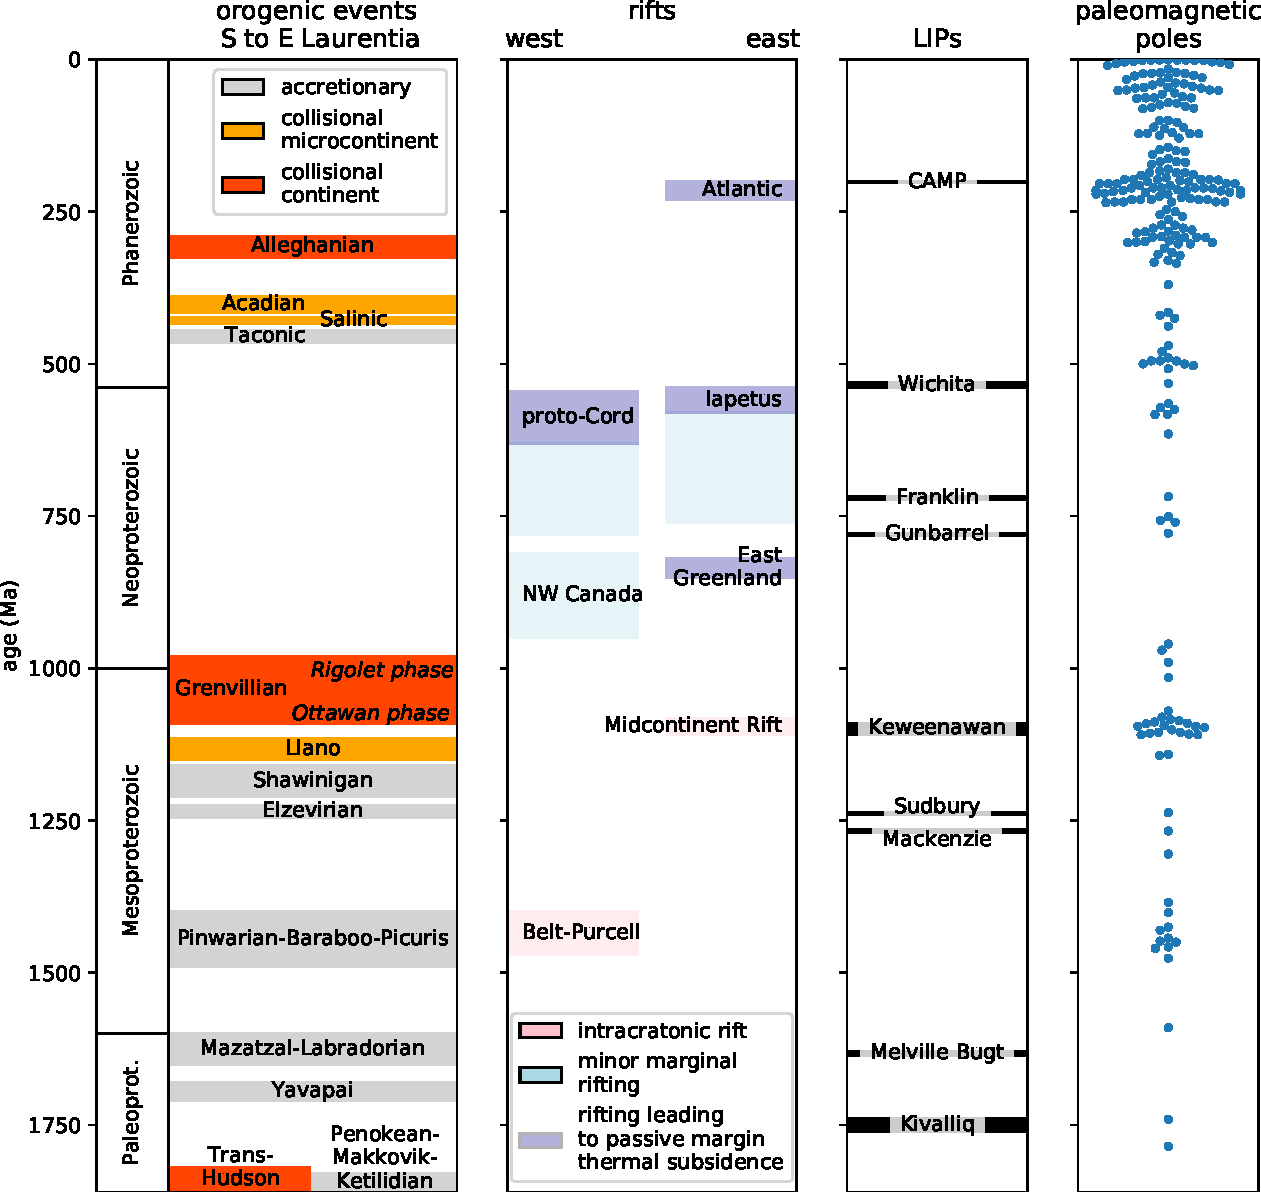
\includegraphics[width=\textwidth]{../Figures/Fig2_Tectonic_history.pdf}
\caption{\textbf{Simplified timeline of Laurentia's tectonic history over the past 1.8 billion years.} Brief summaries and references related to the orogenic and rifting episodes are given in the text. A timeline of large igneous provinces (LIPs) associated with typically brief and voluminous (or interpreted to be voluminous) magmatism is also shown. The interpreted ages of paleomagnetic poles for Laurentia (not including separated terranes) compiled in this study for the Proterozoic (Table 2) and in \cite{Torsvik2012a} for the Phanerozoic is shown. Abbreviations on the figure: CAMP -- Central Atlantic Magmatic Province; proto-Cord -- proto-Cordilleran.}
\label{fig:tectonic_history}
\end{figure*}

Accretionary orogenesis continued locally along the southeastern margin of Laurentia with the amalgamation and accretion of arcs and back-arcs associated with the ca. 1.25 to 1.22 Ga Elzevirian orogeny \citep{Carr2000a,McLelland2013a}. The subsequent ca. 1.19 to 1.16 Ga Shawinigan orogeny is interpreted to be due to the collision and accretion of a previously rifted fragment of Laurentia that led to obduction of the Pyrites Complex ophiolite \citep{Carr2000a,McLelland2010a, Chiarenzelli2011a}. The Shawinigan orogeny is followed by a period of tectonic quiescence on the eastern margin of Laurentia until the collisional orogenesis of the Grenvillian orogeny \citep{McLelland2010a}. An exception to this quiescence during the interval between the Shawinigan and Grenvillian orogenies is ca. 1.15 to 1.12 Ga orogenesis in the Llano uplift of the southern Laurentia margin \citep{Mosher1998a}. Llano orogenesis is interpreted to have resulted from collision of continental lithosphere along with an accreted arc \citep{Mosher1998a}. This orogenesis is earlier and temporally distinct from the Grenvillian orogeny, is only known from a limited spatial area, and is located in a region that experienced further orogenesis during the Grenvillian orogeny \citep{Grimes2004a}. Taken together, this context is suggestive of a microcontinent collision leading to Llano orogenesis prior to terminal Grenvillian continental collision. If this interpretation is correct, it would be similar to Paleozoic orogenesis along the margin where microcontinent collision resulted in the Acadian orogeny prior to Alleghanian orogenesis during the Appalachian orogenic interval (Fig. \ref{fig:tectonic_history}).

The Grenvillian orogeny was a protracted interval of continent-continent collision (ca. 1.09 to 0.98 Ga) leading to amphibolite to granulite facies metamorphism throughout the orogen \citep{Carr2000a, Rivers2008a, Rivers2012a, Indares2020a}. Note that while the terms Grenvillian orogeny and Grenville belt have been used rather loosely in the literature to refer to any late Mesoproterozoic orogenic belt, the timeline of orogenesis on the Laurentia margin has more nuanced constraints than this usage. Properly referring to the Grenvillian orogeny as distinct from the Elzevirian and Shawinigan orogenies enables the available constraints to be comparatively assessed when evaluating potential conjugate continents to Laurentia associated with the orogen (Fig. \ref{fig:tectonic_history}). Evidence of large-scale continent-continent collision at the time of the Ottawan Phase of the Grenvillian orogeny is recorded in Texas \citep{Grimes2004a}, through the Blue Ridge Appalachian inliers \citep{Johnson2020a}, through Ontario and to the Labrador Sea \citep{Rivers2008a, Rivers2012a}. The orogeny is interpreted to have resulted in the development of a thick plateau associated with the Ottawan orogenic phase (ca. 1090 to 1030 Ma; \citealp{Rivers2008a}). Continued convergence during the Rigolet phase of the Grenvillian orogeny led to the development of the Grenville Front tectonic zone and ended ca. 980 Ma \citep{Hynes2010a}.

In the latest Mesoproterozoic (ca. 1.11 to 1.08 Ga) prior to the Grenvillian orogeny, a major intracontinental rift co-located with a large igneous province formed in Laurentia's interior, leading to extension within the Archean Superior province and adjacent Paleoproterozoic provinces to the south (MCR in Fig. \ref{fig:Laurentia_map}; \citealp{Cannon1992b}). This Midcontinent Rift is associated with the emplacement of a thick succession of volcanics and mafic intrusions that are well-preserved in Laurentia's interior. Midcontinent Rift development ceased as major collisional orogenesis of the Grenvillian orogeny began \citep{Cannon1994a, Swanson-Hysell2019a}.

There is significantly less preserved Mesoproterozoic crust on the western margin of Laurentia (Fig. \ref{fig:Laurentia_map}) and the tectonic history through the Mesoproterozoic Era is not as well constrained as on the southern to eastern margin. There are thick successions of Paleoproterozoic siliciclastic and carbonate sedimentary rocks such as the ca. 1.66 to 1.62 Ga Wernecke Supergroup in Yukon, Canada \citep{Delaney1986a, Furlanetto2016a}. The Wernecke Supergroup is interpreted to have resulted from rifting followed by passive margin thermal subsidence \citep{Furlanetto2016a}, although the tectonic setting is poorly understood and could be intracratonic. These metasedimentary rocks were deformed and metamorphosed during the ca. 1.60 Ga Racklan-Forward orogeny that is interpreted to be associated with collision of an arc terrane and potentially a conjugate continent \citep{Thorkelson2005a, Furlanetto2013a, Furlanetto2016a}. Further south along Laurentia's western margin, sedimentary rocks of the 15 to 20 km thick Belt-Purcell Supergroup are associated with a ca. 1.47 to 1.40 rift \citep{Evans2000c}. While the rift is typically interpreted as being intracontinental \citep{Lydon2004a}, the tectonic setting in which it formed is debated. \citet{Hoffman1989c} proposed that it may be a remnant back-arc basin trapped within a continent, while others have envisioned it being associated with continental rifting associated with separation of a conjugate continent \citep{Jones2015a}. This region was subsequently deformed during the ca. 1.37 to 1.33 Ga East Kootenay orogeny that is constrained by granite crystallization and authigenic monazite dates \citep{McMechan1982a, Nesheim2012a, McFarlane2015a}.

Taken together, this late Paleoproterozoic and Mesoproterozoic tectonic history provides significant constraints on paleogeographic reconstructions. In particular, the long-lived history of accretionary orogenesis along the southeast (present-day coordinates) of Laurentia from the initiation of the Yavapai orogeny (ca. 1.71 Ga) to the end of the Shawinigan orogeny (ca. 1.16 Ga) requires a long-lived open margin without a major conjugate continent until the time of terminal Grenvillian collisional orogenesis \citep{Karlstrom2001a}. This constraint is incorporated into paleogeographic models such as that of \citet{Zhang2012a} and \citet{Pehrsson2015a} which maintain a long-lived convergent margin throughout the Mesoproterozoic, but in some reconstructions other continental blocks are reconstructed into positions that are seemingly incompatible with this record of accretionary orogenesis (e.g. Amazonia in \citealp{Elming2009a, Elming2021a}). The great extent of the high-grade metamorphism associated with the Ottawan phase of the Grenvillian orogeny itself strongly suggests a collision between Laurentia and another continent ca. 1080 Ma --- the geological observation of which first led to the formulation of the hypothesis of the supercontinent Rodinia \citep{Hoffman1991a}. This extensive and major collisional orogenesis on Laurentia's margin, and that of other Proterozoic continents, remains a strong piece of evidence that a supercontinent or (proto)supercontinent formed at the 1.0 Ga Mesoproterozoic to Neoproterozoic transition.

\subsubsection{Neoproterozoic rifting}

The subsequent Neoproterozoic tectonic history of Laurentia is dominantly a record of rifting (Fig. \ref{fig:tectonic_history}). Along the western margin of Laurentia, by ca. 760 Ma there was rifting leading to deposition in basins from the Death Valley region of southwestern Laurentia to the Ogilvie Mountains of northwestern Laurentia \citep{Macdonald2013a, Strauss2015a, Dehler2017a, Rooney2017a}. The emplacement of the ca. 780 Ma Gunbarrel large igneous province \citep{Harlan2003a} along this margin and the subsequent extension recorded in the western Laurentia basins is commonly interpreted to be associated with the break-up of Laurentia and a conjugate continent to the western margin (e.g. \citealp{Li2008a}) although this interpretation is difficult to reconcile with the subsequent history of basin development. Extensional basin development continued into the Cryogenian Period with active normal faulting occurring during the deposition of both Sturtian (ca. 717 to 656 Ma) and Marinoan (ca. 645 to 635 Ma) glacial deposits in southwestern Laurentia \citep{Yonkee2014a, Nelson2020a}. Additionally, Cryogenian volcanics along the western Laurentia margin (e.g. \citealp{Eyster2018a}) are interpreted to be the result of active rifting.  A puzzlingly feature of this record of active rifting is that it significantly predates interpreted passive margin thermal subsidence closer to the ca. 539 Ma Neoproterozoic-Phanerozoic boundary that has been linked to lithospheric thinning \citep{Bond1984a, Levy1991a}. If the interpretation of a conjugate continent rifting off the margin prior to the ca. 717 Tonian-Cryogenian boundary is correct, it is unclear why there would be minimal thermal subsidence until the Ediacaran (after 635 Ma in \citealp{Levy1991a}). While the geological evidence supports prolonged extensional tectonism along the western margin of Laurentia,  it suggests that significant lithospheric thinning occurred later than the timing of rifting typically implemented in models of Rodinia break-up. One explanation is that Tonian extensional basin development was associated with transtension in a dominantly strike-slip tectonic regime \citep{Smith2015b, Strauss2015a}. The record of Neoproterozoic basin development led \cite{Yonkee2014a} to propose that the early ca. 780 Ma rifting was intracratonic and that while it may have led to some associated thermal subsidence, there was a second interval of rifting and thermal subsidence associated with Australia rifting away in the Ediacaran (later than in most models). Another possibility, along the lines of the tectonic scenarios proposed by \citet{Ross1991a} and \citet{Colpron2002a}, is that ca. 760 Ma extensional tectonism is an inboard record of rifting and passive margin development that dominantly occurred further to the west. In this model, subsequent continental rifting that drove lithospheric thinning, perhaps associated with the departure of a ribbon continent rather than an already departed major conjugate continent, would be the cause of Ediacaran to Cambrian thermal subsidence.

In northwestern Laurentia from the Ogilvie Mountains (Yukon, Canada) to Victoria Island (Nunavut, Canada), the sedimentary rock record is distinct from that further south as it also records earlier Neoproterozoic basin development during the Tonian Period in addition to Cryogenian basin development \citep{Macdonald2012a}. Lithospheric extension is interpreted from basin development that accommodated deposition of the lower Fifteenmile Group with maximum depositional ages of ca. 1050 Ma with ongoing basin development ca. 812 Ma (age constraint from a U-Pb zircon date on a tuff within the upper Fifteenmile Group; \citealp{Macdonald2010a}) that may have been accommodated through thermal subsidence \citep{Macdonald2012a}. Earlier basin development in the region recorded by the Mesoproterozoic/Neoproterozoic Pinguicula Group could provide valuable insight on the tectonic history as it has been interpreted to have been deposited in an extensional basin \citep{Medig2016a}, however it is poorly constrained in terms of age --- older than the Fifteenmile Group and younger than the ca. 1382 Ma Hart River sills (which themselves have been interpreted to be emplaced in conjunction with rifting; \citealp{Verbaas2018a}). As in southwestern Laurentia, extensional basin development continued into the Cryogenian and Ediacaran which accommodated deposition of the Windermere Supergroup \citep{Moynihan2019a}. Ediacaran rifting transitioned to thermal subsidence in the Cambrian and an early Paleozoic passive margin \citep{Moynihan2019a}. The record of Neoproterozoic basin development on the northern Franklinian margin of Laurentia is more difficult to resolve given the truncation of the margin by the Paleozoic Ellesmerian orogeny \citep{Cocks2011a}. The North Slope terrane of Arctic Alaska is considered to have been part of northeastern Laurentia in the Neoproterozoic and shows a similar history of Tonian to Cryogenian extensional tectonism with limited overall lithospheric stretching that was followed by Ediacaran to early Cambrian extension that led to passive margin sedimentation \citep{Strauss2019a}. 

Another margin that experienced rifting and associated passive margin thermal subsidence earlier in the Neoproterozoic is the northeastern Greenland margin, including the displaced terrane of northeastern Svalbard, Norway (Fig. \ref{fig:tectonic_history}). Available geochronological constraints and thermal subsidence modeling indicate ca. 850 to 820 Ma rifting followed by thermal subsidence of a stable carbonate platform \citep{Maloof2006a, Sonderholm2008a, Halverson2018a}. These data suggest that conjugate continental lithosphere rifted away from northeastern Greenland by ca. 820 Ma although some models place northeastern Greenland in a distal backarc setting \citep{Malone2014a}.

Extensive rifting followed by thermal subsidence occurred along the southeastern to eastern Laurentia margin in the time leading up to the Neoproterozoic-Phanerozoic boundary and is interpreted to be associated with the opening of the Iapetus ocean. On the southern part of the eastern margin, a record of this rifting is preserved as rift basins that were part of failed arms (Rome trough, Reelfoot rift and Oklahoma aulacogen; Fig. \ref{fig:Laurentia_map}) as well as prolonged Cambrian to Ordovician passive margin thermal subsidence along the margin \citep{Bond1984a, Whitmeyer2007a}. The ages of igneous intrusions that have been interpreted to be rift-related play a significant role in interpretations of this history such as in the rift development model of \citet{Burton2010a}. In this model, spatially-restricted rifting occurs ca. 760 to 680 Ma in the region of present-day North Carolina and Virginia. Rifting initiated in the region from present-day New York to Newfoundland ca. 620 to 580 Ma associated with the Central Iapetus Magmatic Province (CIMP; Fig. \ref{fig:Grenville_reconstructions}) and by ca. 580 to 550 Ma rifting extended along the length of Laurentia's eastern margin. The last phase of this rifting has been interpreted to be associated with the separation of the Argentine pre-Cordillera Cuyania terrane ca. 540 Ma \citep{Dickerson1998a, Martin2019a}.

As with other rifted margins, it is difficult to distinguish the separation of a cratonic fragment as a microcontinent from the rifting and departure of a major craton, as the record that lingers on the craton is similar. Recognizing this ambiguity, it has been proposed that rather than being associated with spatially-restricted or failed rifting, ca. 700 Ma extension (which occured in the southern part of the eastern margin) was associated with breakup and separation of a conjugate continent and that there was subsequent rifting of smaller terranes off the eastern Laurentia margin ca. 600 Ma \citep{Chew2008a, Escayola2011a, Robert2020a}. In these models, the separation of a conjugate continent ca. 700 Ma leads to the formation of an ocean termed the Puncoviscana Ocean by \citet{Escayola2011a} and the Paleo-Iapetus Ocean by \citet{Robert2020a}. The subsequent rifting of terranes off the Laurentia margin ca. 600 Ma would have resulted in the formation of the (Neo-)Iapetus Ocean and the record of thermal subsidence associated with passive margin development on Laurentia \citep{Escayola2011a, Robert2020a}.

\subsubsection{Similarities in Laurentia's Proterozoic and Phanerozoic tectonic histories}

The eastern margin of Laurentia then went through multiple phases of Appalachian orogenesis. As is visualized in Figure \ref{fig:tectonic_history}, there are parallels between the Grenville and Appalachian orogenic intervals in that in both cases there was a period of arc-continent collision (Elzevirian orogeny in the Grenville interval; Taconic orogeny in the Appalachian interval) followed by microcontinent accretion (Shawinigan/Llano orogenies in the Grenville interval; Acadian orogeny in the Appalachian interval) that culminated in large-scale continent-continent collision (Grenvillian orogeny in the Grenville interval; Alleghanian orogeny in the Appalachian interval). These similarities are the consequence of an active margin facing an ocean basin that was progressively consumed until continent-continent collision. In the case of the Grenville interval, this terminal collision is interpreted to be associated with the assembly of the supercontinent Rodinia, and in the Appalachian interval it is interpreted to be associated with the assembly of the supercontinent Pangea.

Even without considering other continents on Earth, the geological record of Paleoproterozoic collision of Archean provinces combined with accretionary orogenesis at that time and through the rest of the Paleoproterozoic and Mesoproterozoic Eras provides strong evidence for mobile plate tectonics driving Laurentia's evolution throughout the past 2 billion years. This tectonic history inferred from geological data can be enhanced through integration with the paleomagnetic record.

\subsection{Paleomagnetic pole compilation}

\begin{figure*}
\centering
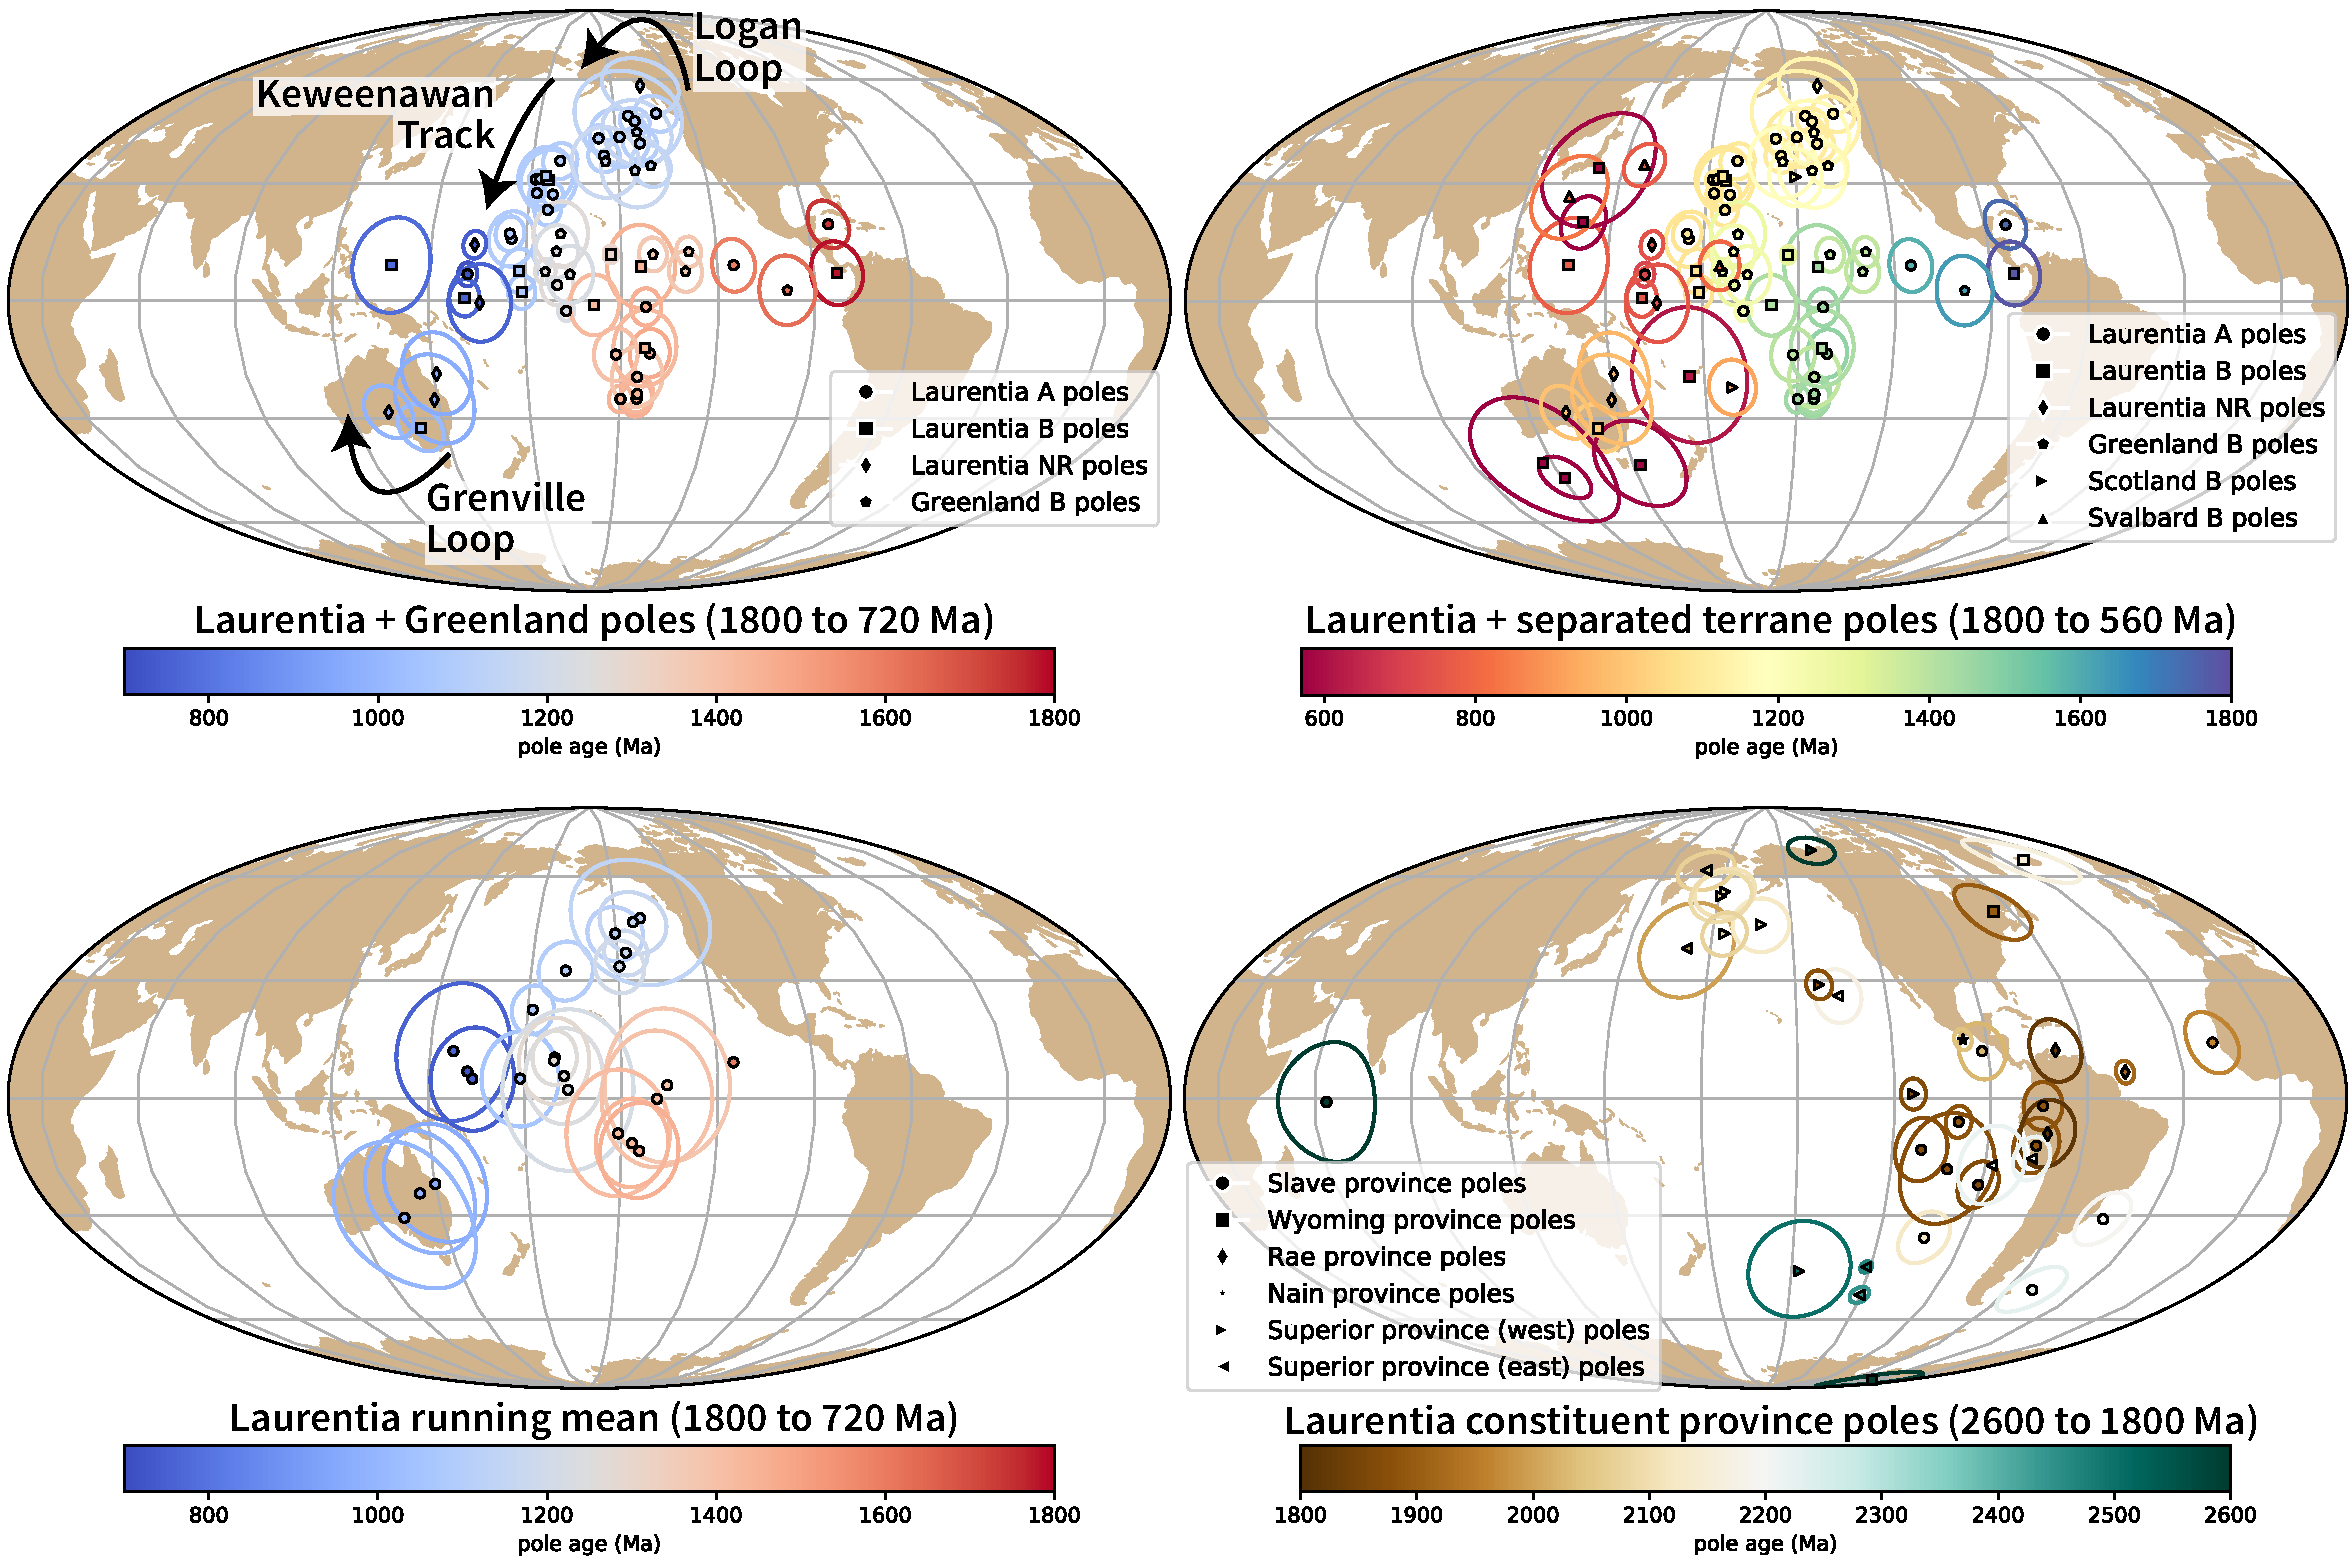
\includegraphics[width=\textwidth]{../Figures/Fig3_Laurentia_poles_combined.pdf}
\caption{\textbf{Paleomagnetic poles from Laurentia.} Upper-left panel: Paleomagnetic poles from 1800 to 720 Ma for Laurentia (including Greenland). Portions of the apparent polar wander path (APWP) are referred to by the names Logan loop, Keweenawan track, and Grenville loop in the literature and those are labeled next to the associated poles. Upper-right panel:  Paleomagnetic poles from 1800 to 580 Ma for Laurentia (including those from the separated terranes of Greenland, Scotland and Svalbard rotated to Laurentia coordinates). The youngest poles from the Ediacaran Period have unusually variable positions as discussed in the text. Lower-left panel: Running mean APWP calculated with a 20 million year moving window. Lower-right panel: Poles for the Archean provinces of Laurentia prior to Laurentia's Paleoproterozoic amalgamation.}
\label{fig:Laurentia_poles}
\end{figure*}

In this chapter, I focus on the compilation of paleomagnetic poles developed through the Nordic Paleomagnetism Workshops with some additions and modifications (Fig. \ref{fig:Laurentia_poles} and Table 2). The Nordic Paleomagnetism Workshops have taken the approach of using expert panels to assess paleomagnetic poles and assign them grades to convey the confidence that the community has in these results \citep{Evans2021a}. While many factors associated with paleomagnetic poles can be assessed quantitatively through Fisher statistics and the precision of geochronological constraints, other aspects such as the degree to which available field tests constrain the magnetization to be primary require expert assessment. The categorizations used by the expert panel are `A' and `B' with the last panel meeting occurring in Fall 2017 in Leirubakki, Iceland \citep{Brown2018a}. The `A' rating refers to poles that are judged to be of such high quality that they provide essential constraints that should be satisfied in paleogeographic reconstructions. The `B' rating is associated with poles that are judged to likely provide a high-quality constraint, but have some deficiency such as remaining ambiguity in the demonstration of primary remanence or the quality/precision of available geochronologic constraints. In addition, in this chapter I refer to select additional poles that were not given an `A' or `B' classification at the Nordic Workshops as not-rated (`NR'). These additional poles are taken from the Paleomagia database \citep{Veikkolainen2014a} in conjunction with the papers in which they were reported. Many additional poles in the database to those that are rated are valuable and should not be dismissed from being considered in paleogeographic reconstructions. However, there are ambiguities associated with many of the poles not given Nordic `A' or `B' ratings in terms of how well the nature of the remanence is constrained, including its age. For example, there are many poles that have been developed from lithologies of the Trans-Hudson orogen (e.g. \citealp{Symons2005a}). However, these poles typically lack field tests, have poor control on paleohorizontal and are hypothesized to suffer from variable overprints as discussed in \cite{Raub2008a} and \cite{DAgrella-Filho2020a}. Given the preponderance of similar directions, three representative poles from the Trans-Hudson orogen are included in the Nordic Workshop compilation (Table 2) as `B' rated poles. However, they should be used with caution given that they suffer from the same deficiencies. 

There are similar issues with the rich data sets associated with intrusive and metamorphic lithologies of the Grenville Province that are the available paleomagnetic constraints for Laurentia at the Mesoproterozoic-Neoproterozoic boundary. The ages of the remanence associated with these poles is complicated by the reality that the magnetization was acquired during exhumation and associated cooling within the Grenville orogen. Cooling ages of deeply exhumed lithologies are more difficult to robustly constrain than the ages of remanence associated with dated eruptive units or shallow-level intrusions. As a result, the vast majority of Grenville Province poles are not given an `A' or `B' rating with the exception of the `B' rated pole from the ca. 1015 Ma Haliburton intrusions (Table 2). However, while any one of these Grenville poles could be interpreted to suffer from large temporal uncertainty, the overall preponderance of poles in a similar location at the time suggests that they need to be taken seriously within paleogeographic reconstructions of Laurentia (although an alternative view of an allochthonous origin put forward by \citealp{Halls2015a} is discussed below). In this compilation, the poles of \cite{Brown2012a} from the Adirondack highlands for which the magnetic mineralogy and associated relative ages of remanence are relatively well-constrained are included (Table 2). Additional not-rated poles, published after the ratings were conferred, that are included in the present compilation are: 1) a pole from the ca. 1780 Ma East Central Minnesota Batholith that confirms that the Slave, Hearne, Rae, and Superior provinces were part of coherent amalgamated Laurentia following the Trans-Hudson orogeny \citep{Swanson-Hysell2021a}; 2) a pole for the ca. 1144 Ma Ontario lamprophyre dikes \citep{Piispa2018a} that strengthens the position of Laurentia at that time and coincides with the position of the poles from the ca. 1140 Ma Abitibi dikes \citep{Ernst1993a}. These poles will likely receive an `A' rating when assessed at the next Nordic paleomagnetism workshop. Poles from the Neoproterozoic Chuar Group of southwestern Laurentia (ca. 760 Ma)  as presented in \cite{Eyster2020a}, incorporating data from \cite{Weil2004a}, are also included. 

\subsection{Differential motion before Laurentia amalgamation}

Prior to the termination of the Trans-Hudson orogeny (before 1.8 Ga), paleomagnetic poles need to be considered with respect to the individual Archean provinces. For the Superior province, an additional complexity is that paleomagnetic poles from Siderian to Rhyacian Period (2.50 to 2.05 Ga) dike swarms, as well as deflection of dike trends, support an interpretation that there was substantial Paleoproterozoic rotation of the western Superior province relative to the eastern Superior province across the Kapuskasing Structural Zone \citep{Bates1991a, Evans2010a}. This interpretation is consistent with the hypothesis of \citet{Hoffman1988a} that the Kapuskasing Structural Zone represents major intracratonic uplift related to the Trans-Hudson orogeny. \cite{Evans2010a} propose an Euler rotation of (51\textdegree N, 85\textdegree W, -14\textdegree CCW) to reconstruct western Superior relative to eastern Superior and interpret that the rotation occurred in the time interval of 2.07 to 1.87 Ga.  I follow this interpretation and group the poles into Superior (West) and Superior (East).

\begin{figure*}
\centering
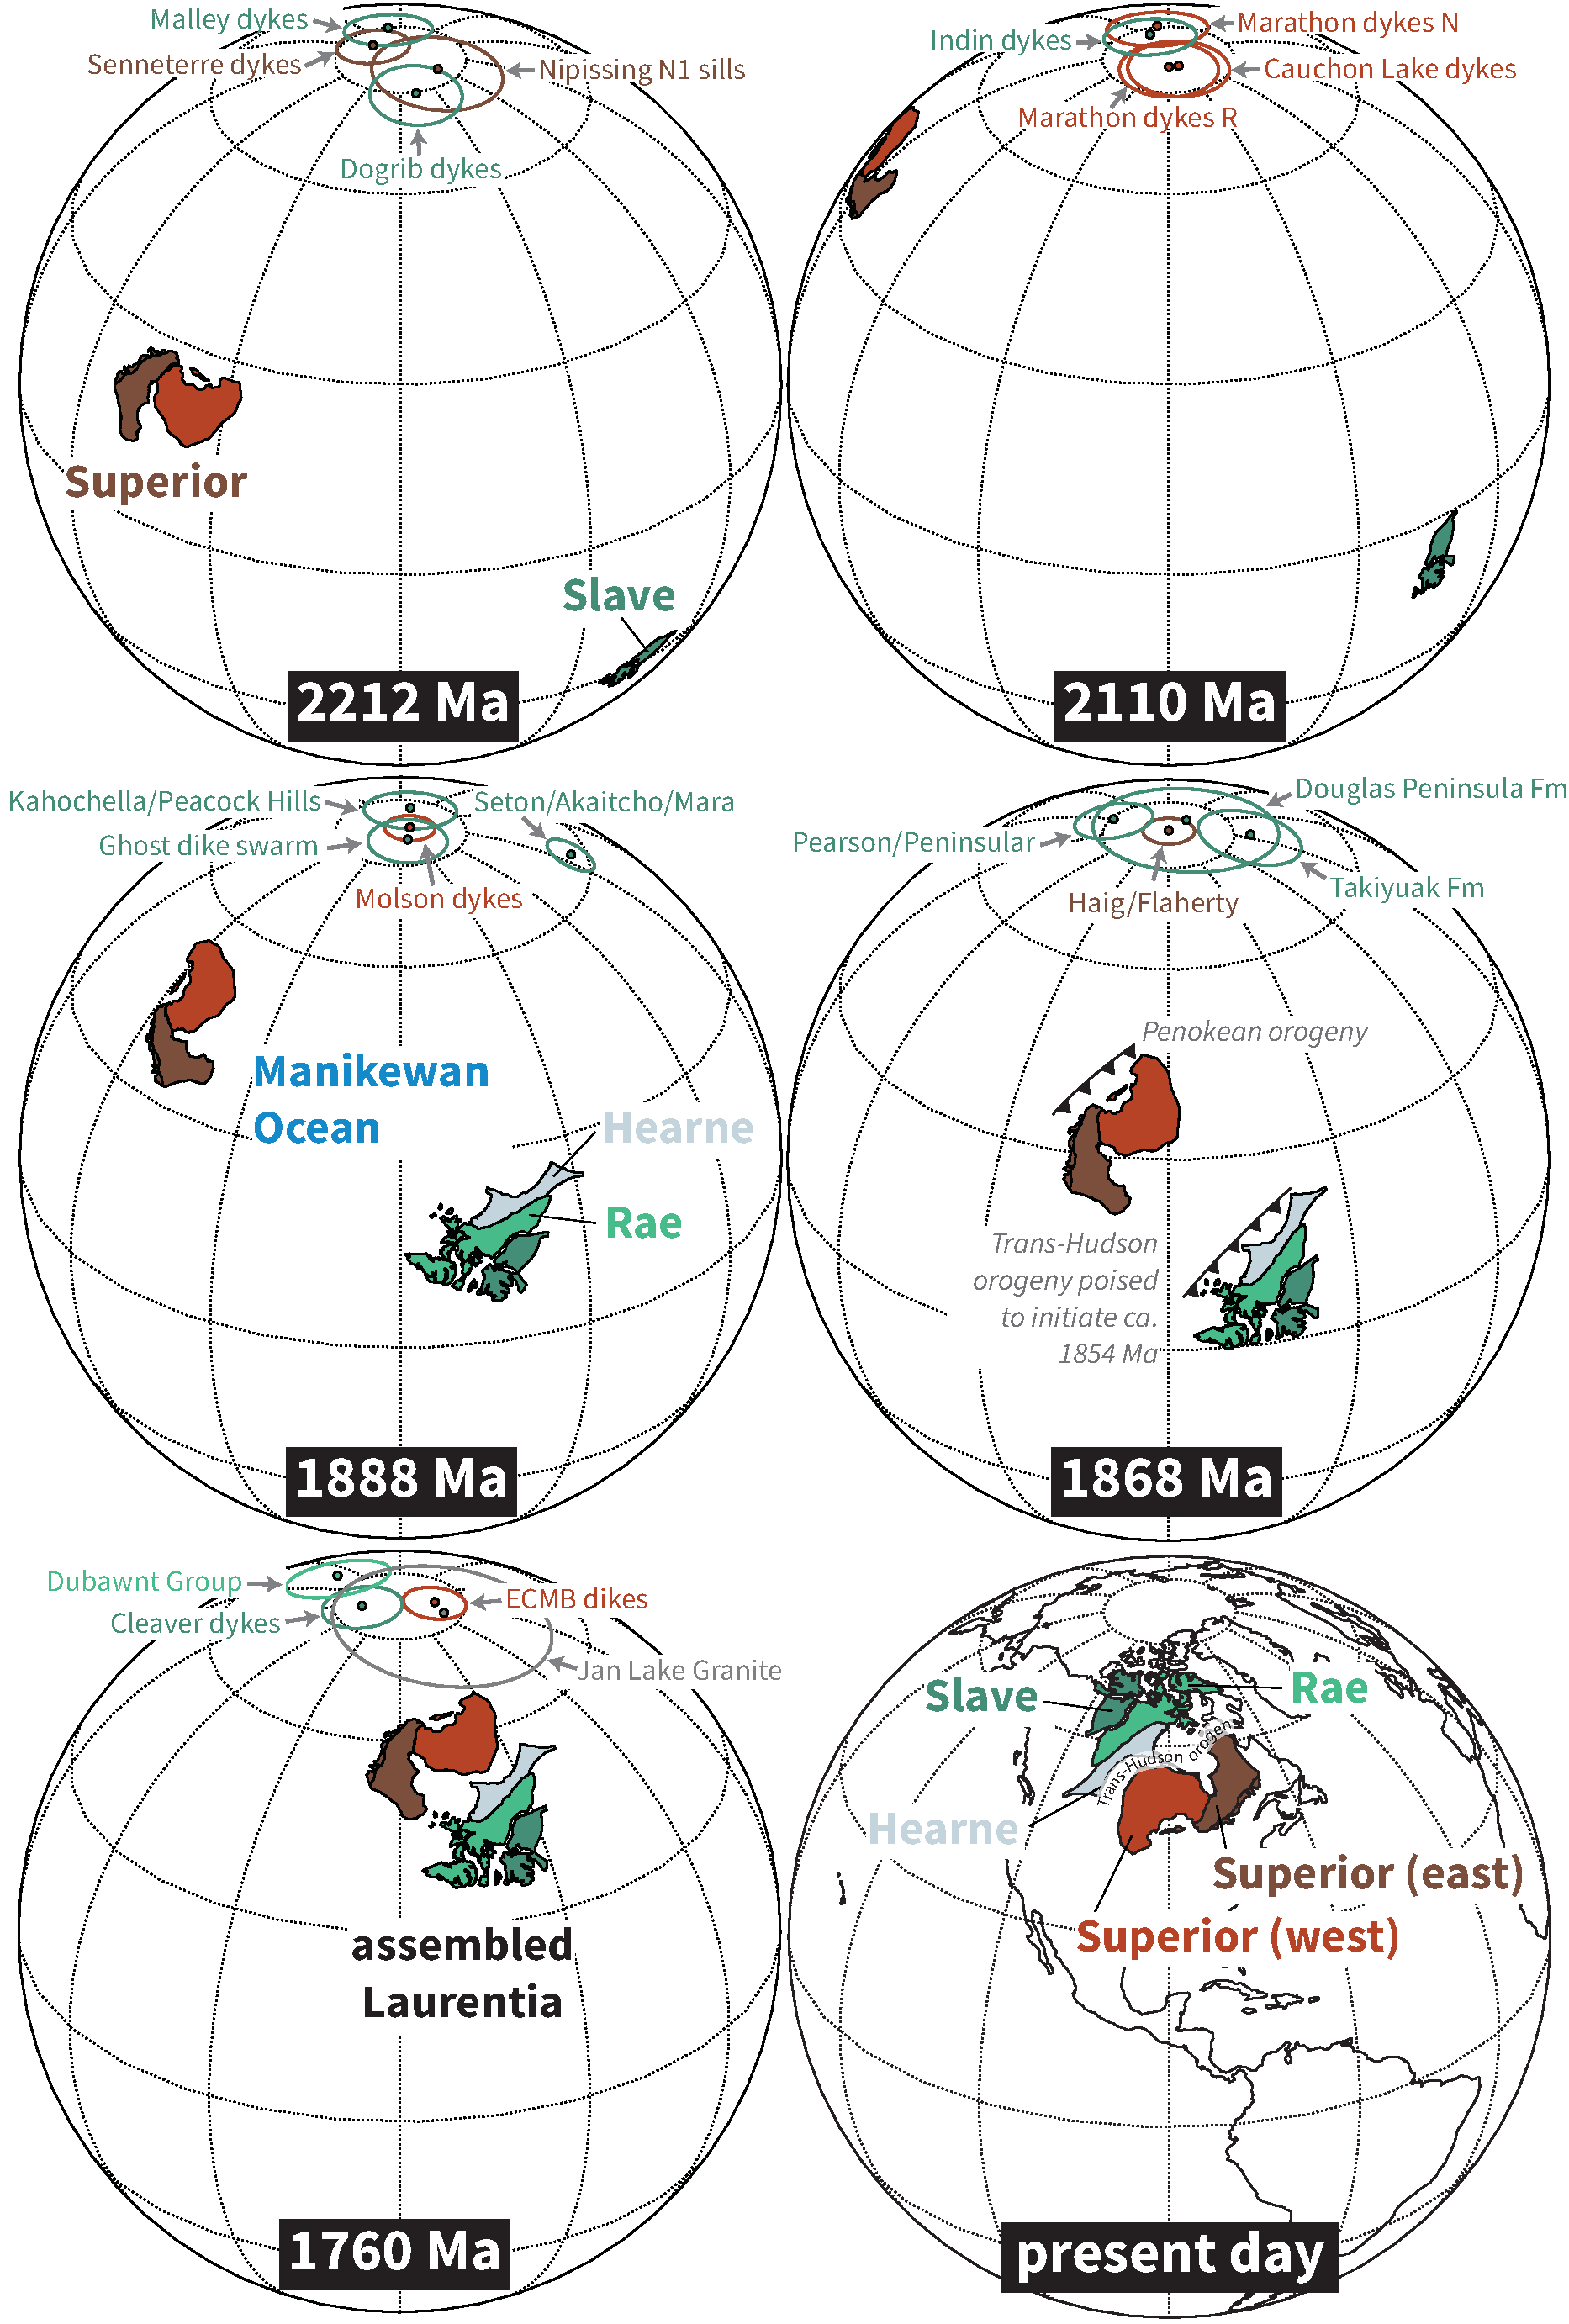
\includegraphics[width=5.25 in]{../Figures/Fig4_Superior_Slave_reconstructions.pdf}
\caption{\textbf{Paleogeographic reconstructions developed using poles from the Superior, Slave and Rae provinces.} The polarity options that are chosen for the provinces are those that minimize total apparent polar wander path length. This model follows \cite{Swanson-Hysell2021a} and reconstructs a wide Manikewan ocean that underwent orthogonal closure rather than an alternative possibility of a narrower Manikewan ocean with a pivot-like closure. Paleomagnetic poles are shown colored to match their respective province with these provinces shown in present-day coordinates and labeled in the 0 Ma panel. Poles with ages that are within 20 million years of the given time slice are shown. The relatively well-resolved pole paths from the Superior and Slave provinces (Fig. \ref{fig:Laurentia_poles}) that are utilized for these reconstructions provide strong support for differential plate tectonic motion between 2220 and 1850 Ma.}
\label{fig:Superior_Slave_recons}
\end{figure*}

There are poles in the compilation for the Slave, Wyoming, Rae, Superior and North Atlantic provinces prior to Laurentia amalgamation (Fig. \ref{fig:Laurentia_poles} and Table 2). Overall, these data provide an opportunity to re-evaluate the paleomagnetic evidence for relative motions between Archean provinces prior to Laurentia assembly. A lingering question raised in \citet{Hoffman1988a} is to what extent the Archean provinces each had independent drift histories with significant separation or shared histories before experiencing fragmentation and reamalgamation. The strongest analysis in this regard comes from comparisons between paleomagnetic poles between the Superior and Slave provinces \citep{Buchan2009a, Mitchell2014a, Buchan2016a}. High-quality paleomagnetic poles from these two provinces provide strong support for differential motion between the Superior and Slave provinces between 2.2 and 1.8 Ga with the two provinces not being in their present-day relative orientation to one another and having distinct pole paths as constrained by five time slices of nearly coeval poles between 2.23 and 1.89 Ga (Fig. \ref{fig:Superior_Slave_recons}; \citealp{Buchan2016a}). These data provide paleomagnetic support for the Superior and Slave provinces having independent histories of differential motion. The data also support the hypothesis that the Trans-Hudson orogeny is the result of terminal collision associated with the closure of the Manikewan Ocean between the Superior province and the Hearne+Rae+Slave provinces. Reconstructions developed for this chapter of the Superior and Slave provinces using these poles are shown in Figure \ref{fig:Superior_Slave_recons} and illustrate the difference in implied orientation and paleolatitude that results from these well-constrained poles.

\subsection{Paleogeography of an assembled Laurentia}

Following the amalgamation of the Archean provinces in Laurentia by ca. 1.8 Ga, poles from each part of Laurentia can be considered to reflect the position of the entire composite craton. This interpretation of a coherent Laurentia is confirmed paleomagnetically by the consistent positions of ca. 1780 to 1740 Ma poles from the Slave, Hearne/Rae, and Superior Provinces (Fig. \ref{fig:Superior_Slave_recons}; \citealp{Swanson-Hysell2021b}). It is worth considering the possibility that poles from zones of Paleoproterozoic and Mesoproterozoic accretion could be allochthonous to the craton. \cite{Halls2015b} argued that this was the case for late Mesoproterozoic and early Neoproterozoic poles from east of the Grenvillian allochthon boundary fault. However, the majority of researchers have considered these poles to post-date major differential motion and be associated with cooling during collapse of a thick orogenic plateau developed during continent-continent collision (e.g. \citealp{Brown2012a}). Poles with a B-rating are also included in the compilation that come from Greenland, Svalbard and Scotland. These terranes were once part of contiguous Laurentia, but have subsequently been separated through translation and rifting. These poles need to be rotated into the Laurentia reference frame prior to use for tectonic reconstruction, and I apply the rotations shown in Table \ref{tab:terrane_rotations}. The Euler pole and rotation is quite well-constrained for Greenland as it is associated with recent opening of Baffin Bay and the Labrador Sea (for which the rotation of \citealp{Roest1989a} is used). The reconstruction of Scotland is associated with the opening of the Atlantic (for which the rotation employed by \citealp{Torsvik2017a} is used) which is well-constrained, but has more uncertainty associated with the Euler pole than that for Greenland. The reconstruction of Svalbard is more challenging and non-unique given a multi-stage tectonic history involving both translation within the Caledonides and subsequent rifting. The preferred Euler pole parameters of \cite{Maloof2006a} are used here for this reconstruction. This Euler rotation is designed, in particular, to honor the high degree of similarity between Tonian sediments in East Greenland and those of East Svalbard \citep{Maloof2006a, Hoffman2012a} and to reconstruct East Svalbard to be aligned with these correlative sedimentary rocks.

\begin{table}[hbt]
\caption{Rotations of separated terranes}
{\scriptsize
\begin{tabular}{|l|l|l|l|p{1.1 in}|}
  \hline
& Euler pole & Euler pole & rotation & note and \\
Terrane & longitude & latitude & angle & citation \\
\hline
Greenland & -118.5 & 67.5 & -13.8 & Cenozoic separation of Greenland from Laurentia associated with opening of Baffin Bay and the Labrador Sea \citep{Roest1989a} \\
\hline
Scotland & 161.9 & 78.6 & -31.0 & Reconstruction of Atlantic Ocean opening following \cite{Torsvik2017a} \\
\hline
Svalbard & 305.0 & 81.0 & -68 & Rotate Svalbard to Laurentia in fit that works well with East Greenland basin according to \cite{Maloof2006a}\\
\hline
\end{tabular}
}
\label{tab:terrane_rotations}
\end{table}

Through the Proterozoic, there are intervals where there are abundant paleomagnetic poles that constrain Laurentia's position and intervals when the record is sparse (shown colored by age in Fig. \ref{fig:Laurentia_poles}). To further visualize the temporal coverage of the poles and to summarize the motion, implied paleolatitudes for an interior point on Laurentia are shown in Figure \ref{fig:Laurentia_paleolatitude}. The ages of the utilized paleomagnetic poles are also shown in comparison to the simplified summary of tectonic events in Figure \ref{fig:tectonic_history}. Both collisional and extensional tectonism can result in the formation of lithologies that can be used to develop paleomagnetic poles either as a result of basin formation, magmatism or both. In addition, intraplate magmatism resulting from plume-related large-igneous provinces (LIPs) can lead to paleomagnetic poles in periods that are otherwise characterized by tectonic quiescence (e.g. the ca. 1267 Ma Mackenzie LIP; Fig. \ref{fig:tectonic_history}). Intracontinental rifts have led to the highest density of poles both in the case of the ca. 1.4 Ga Belt-Purcell Supergroup and the ca. 1.1 Ga Midcontinent Rift (Figs. \ref{fig:Laurentia_map} and \ref{fig:tectonic_history}). The quality and resolution of the record from the Midcontinent Rift is aided by the voluminous magmatism that occurred in conjunction with basin formation that enables the development of a well-calibrated apparent polar wander path \citep{Swanson-Hysell2019a}. The late Tonian Period also has a number of poles including the Gunbarrel LIP (ca. 780 Ma) and Franklin LIP (ca. 720 Ma), as well as similarly-aged sedimentary rocks from western Laurentia basins \citep{Eyster2020a}. Overall, there is internal consistency among the paleomagnetic poles within intervals for which there is high-resolution coverage. These data result in progressive paths (Fig. \ref{fig:Laurentia_poles}) such as ascending to the ca. 1140 to 1108 Ma apex of the Logan Loop \citep{Robertson1971a}, down the ca. 1108 to 1080 Ma Keweenawan Track \citep{Swanson-Hysell2019a} to the ca. 980 Ma Grenville Loop \citep{McWilliams1975a} prior to a temporal gap before the late Tonian (ca. 775 to 720 Ma) path \citep{Eyster2020a}.

Data from other terranes add resolution to the record. In particular, data from Greenland add 12 poles between 1385 and 1160 Ma when there are only four poles from mainland Laurentia. Given that the rotation between Greenland and mainland Laurentia is well-constrained (Table \ref{tab:terrane_rotations}), once rotated these poles can be used for reconstruction of the entire craton. The reliability of this approach gains credence through the good agreement between the ca. 1633 Ma Melville Bugt diabase dikes pole from Greenland \citep{Halls2011a} and the ca. 1590 Ma Western Channel diabase pole of mainland Laurentia (\citealp{Irving1972a}; Figs. \ref{fig:Laurentia_poles} and \ref{fig:Laurentia_paleolatitude}). Similarly, there is good agreement between the ca. 1267 Ma Mackenzie dikes pole of Laurentia \citep{Buchan2000a} and coeval poles from Greenland such as the ca. 1275 Ma North Qoroq intrusives \citep{Piper1992a} and Kungnat Ring dike \citep{Piper1977a}. Furthermore, the Greenland poles with ages that fall between the ca. 1237 Ma Sudbury dikes and ca. 1144 Ma lamprophyre dikes pole of mainland Laurentia are consistent with older and younger constraints from mainland Laurentia while filling in the ascending limb of the path leading up to the apex of 1140 to 1108 Ma poles known as the Logan Loop (Figs. \ref{fig:Laurentia_poles} and \ref{fig:Laurentia_paleolatitude}).

An exception to this overall agreement between coeval poles from Greenland and mainland Laurentia occurs ca. 1382 Ma. There are poles of this age from Greenland associated with the Zig-Zag Dal basalts and related intrusions \citep{Marcussen1983a, Abrahamsen1987a}. However, these poles are in a distinct location from poles of similar age associated with the Belt-Purcell Supergroup (e.g. the McNamara Formation and Pilcher/Garnet Range and Libby Formations; \citealp{Elston2002a}). Additionally, the older Belt-Purcell Supergroup poles form a more southerly population than time-equivalent poles from elsewhere in Laurentia such as the Mistastin Pluton. There are potential complications associated with the Belt-Purcell Supergroup being exposed within thrust sheets with significant Mesozoic and Cenozoic deformation. However, vertical axis rotations of the Belt region are not able to bring the Belt poles into agreement with those from Laurentia or Greenland nor is translation away from the craton. Another potential complication is that the remanence used for the development of the Belt-Purcell Supergroup poles resides in hematite. As a result, there is the potential for inclination-flatting within the sedimentary rocks from which poles are developed. However, applying a moderate inclination correction factor of $f=0.6$ also does not bring the poles into congruence with the Zig-Zag Dal basalts. There is the potential that the hematite could be the result of post-depositional oxidation --- the remanence of the Purcell lavas pole is also held by hematite such that it is a chemical remanent magnetization (potentially acquired soon after eruption) rather than being a thermal remanent magnetization held by magnetite \citep{Elston2002a}. However the overall coherency of the pole directions from the Belt-Purcell Supergroup and the presence of geomagnetic reversals as interpreted from antipodal directions has been taken as evidence that the remanence is primary \citep{Elston2002a}. At present, it is unclear which poles are a better representation of Laurentia's position ca. 1400 Ma.

The interval of the record when there are the most significant inconsistencies between poles of similar age is the Ediacaran Period at the end of the Neoproterozoic Era (Figs. \ref{fig:Laurentia_poles} and \ref{fig:Laurentia_paleolatitude}).  Between 583 and 565 Ma, paleomagnetic poles imply both low-latitude and high-latitude positions of Laurentia  (Fig. \ref{fig:Laurentia_paleolatitude}). This conflicting record is a longstanding problem and has led to the presentation of both high-latitude and low-latitude Laurentia paleogeographic reconstructions at the time (e.g. \citealp{Pisarevsky2001a,Li2008a}). One explanation for these variable pole positions is that they are the result of large-scale oscillatory true polar wander in the Ediacaran where rapid rotation of the entire silicate Earth influenced poles in Baltica and West Africa as well \citep{McCausland2007a, Robert2017a}. Paleodirectional data from single feldspar crystals from the Sept-\^Iles layered intrusion led \cite{Bono2015a} to interpret the lower inclination (and therefore lower latitude) direction from the intrusion (the one included as the ca. 565 Ma Sept-\^Iles pole in Table 2; \citealp{Tanczyk1987a}) as the primary thermal remanent magnetization.  \cite{Bono2015a} interpreted steeper directions also recovered from the intrusives as the result of remagnetization. They suggested that other steep magnetizations from Ediacaran Laurentia plutonic rocks, such as that observed in the ca. 583 Ma Baie des Mountons complex (the A group of \cite{McCausland2011a} in Table 2), are also the result of remagnetization. The lower inclination Baie des Mountons complex B Group directions result in a pole that is indistinguishable from the lower inclination  Sept-\^Iles intrusives pole. Another possibility discussed in the literature is that the lack of congruency between poles in this time interval is due to a particularly weak and non-dipolar geomagnetic field \citep{Abrajevitch2010a, Halls2015a, Bono2019a}. Data from the ca. 585 Ma Grenville dyke swarm of Laurentia, that are interpreted as primary, reveal $\sim$90\textdegree\ differences in direction within dikes dated within 2.5 $\pm$ 0.9 million years of one another \citep{Halls2015a}. The rates of $>$26\textdegree /Myr ($>$288 cm/yr) implied if these data are interpreted as resulting from plate motion or true polar wander were considered as dynamically implausible by \cite{Halls2015a} leading the authors to favor a deviation from axial dipolar behavior as the explanation for disparate Ediacaran directions. Estimates of magnetic paleointensity in these Grenville dikes are anomalously weak \citep{Thallner2020a} as are data from coeval volcanics in Ukraine \citep{Shcherbakova2019a} which could support an anomalous deviation from stable axial dipolar geomagnetic field behavior at the time as interpreted by \cite{Halls2015a}.  Regardless of mechanism, the Ediacaran data stand out as anomalous relative to the coherency of the rest of the poles in the compiled record for Laurentia (Fig. \ref{fig:Laurentia_paleolatitude}). 

\begin{figure*}
\centering
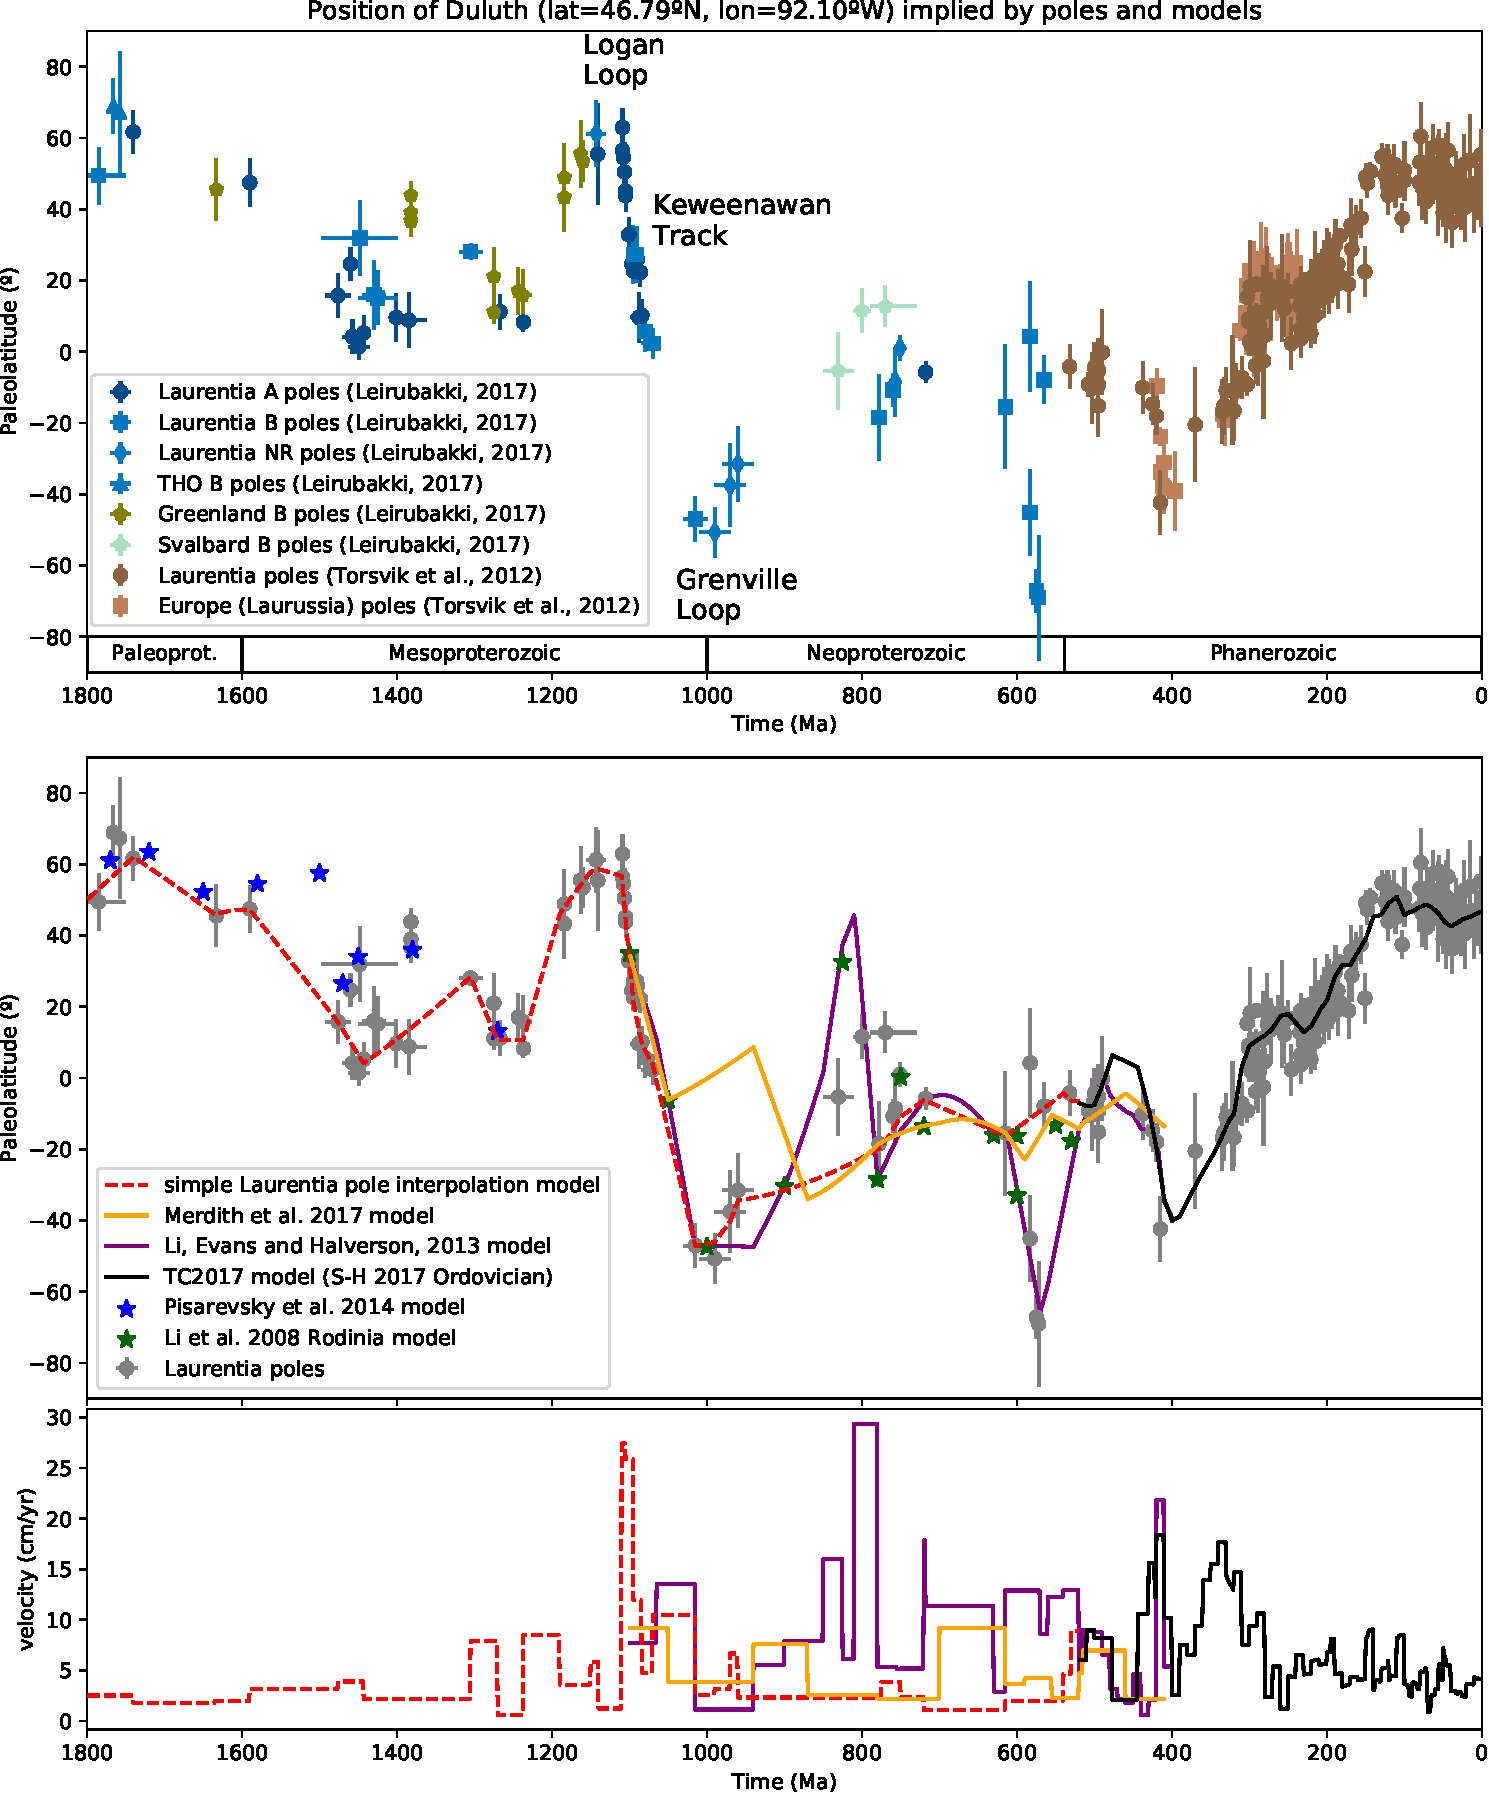
\includegraphics[width=0.9\textwidth]{../Figures/Fig5_Laurentia_paleolatitude.pdf}
\caption{\textbf{Laurentia paleolatitude through time in data and models.} Top panel: Paleolatitude for the city of Duluth on the southern margin of the Superior province (present-day coordinates of lat=46.79\textdegree N, lon=92.10\textdegree W) implied by paleomagnetic poles from Laurentia and associated terranes. The paleomagnetic poles are compiled in Table 2. Middle panel: Paleolatitude implied by Laurentia poles compared with that implied by published paleogeographic models and the simple Laurentia model used in this chapter for the reconstructions in Figure \ref{fig:Laurentia_reconstructions}. TC2017 refers to \cite{Torsvik2017a} and SHM2017 refers to \cite{Swanson-Hysell2017a}. Bottom panel: the velocity implied by the continuous paleogeographic models in cm per year for the Duluth reference point on Laurentia.}
\label{fig:Laurentia_paleolatitude}
\end{figure*}

Synthesizing the compilation of paleomagnetic poles for Laurentia into a composite path over the past 1.8 billion years presents a challenge given the highly variable temporal coverage. The method typically applied in the Phanerozoic is to develop synthesized pole paths either through fitting spherical splines through the data or calculating binned running means where the Fisher mean of poles within a given interval are calculated \citep{Torsvik2012a}. Applying such an approach can reduce the influence of spurious poles. Such synthesis is particularly important in regions of high data density where seeking to satisfy every mean pole position would result in jerky motion.

A synthesized pole path for Laurentia is developed here and used to develop a paleogeographic reconstruction of Laurentia constrained by the compilation of paleomagnetic poles. The paleolatitude implied by this continuous simple Laurentia pole interpolation model is shown in Figure \ref{fig:Laurentia_paleolatitude}. This path is based on Laurentia data alone which means that it is poorly constrained through intervals of sparse data (950-850 Ma for example). One could use interpretations of paleogeographic connections with other cratons (e.g. Baltica in the early Neoproterozoic) to fill in such portions of the path, however the result then becomes model-dependent without being constrained by data from Laurentia itself. In portions of the record with a more dense record of poles, such as ca. 1450 Ma, a calculated running mean is used to integrate constraints from multiple poles (shown in Fig \ref{fig:Laurentia_poles}). This method follows the approach taken in the Phanerozoic (e.g. \citealp{Torsvik2012a}) wherein all poles within a 20 Myr interval are averaged with the interval than progressively moved forward in 10 Myr steps. When there are isolated `A' grade poles without other temporally-similar poles, these poles are fully satisfied in model. Where there are no constraints a simple interpolation between constraints is made. While data from Scotland and Svalbard are associated with Laurentia, the Scotland poles are poorly constrained in time and the Svalbard rotation to Laurentia is uncertain. These poles are not utilized in the simple Laurentia model, which means that the model as shown does not include oscillatory true polar wander interpreted to have occurred ca. 810 and 790 Ma based on data from Svalbard \citep{Maloof2006a}. The model of \cite{Li2013a} shown in Figure \ref{fig:Laurentia_paleolatitude} does seek to partially incorporate this true polar wander while also incorporating an interpretation of the paleomagnetic pole record from South China (albeit one that needs to be revisited given updates to the paleomagnetic and geochronologic record from South China; \citealp{Zhang2021a}).

One downside of a running mean approach is that it pulls the mean to regions of high data density. As was shown in \cite{Swanson-Hysell2019a}, this behavior can reduce motion along an apparent polar wander path. As a result, for the portion of the reconstruction during the interval of time ca. 1110 to 1070 Ma where there is high data density from the Midcontinent Rift, I use the time-calibrated path from \cite{Swanson-Hysell2019a}.

Paleogeographic snapshots for the past position of Laurentia reconstructed using this synthesis of the paleomagnetic poles are shown in Figure \ref{fig:Laurentia_reconstructions}. These reconstructions use the tectonic elements as defined by \citet{Whitmeyer2007a} with these elements being progressively added associated with Laurentia's accretionary growth. As a reminder to the reader, paleomagnetic poles provide constraints on the paleolatitude of a continental block as well as its orientation (which way was north relative to the block). While they provide constraints in this regard, they do not provide constraints in and of themselves for the longitudinal position of the block. Other approaches to obtain paleolongitude utilize geodynamic hypotheses such as assuming that large low shear velocity provinces have been stable plume-generating zones in the lower mantle to which plumes can be reconstructed \citep{Torsvik2014a} or that significant pole motion in certain time intervals is associated with true polar wander axes with specified paleolongitudes that switch through time in conjunction with hypothesized supercontinent cyclicity \citep{Mitchell2012a}. In Figure \ref{fig:Laurentia_reconstructions}, the map projections are centered on the longitudinal position of Duluth with the orientation and paleolatitude of Laurentia being constrained by the paleomagnetic pole compilation as synthesized in the simple pole interpolation model (Fig. \ref{fig:Laurentia_paleolatitude}).

\begin{figure*}
\centering
\includegraphics[width=\textwidth]{../Figures/Fig6_Laurentia_reconstructions.pdf}
\caption{\textbf{Paleogeographic reconstructions of Laurentia at time intervals through the Proterozoic.} These reconstructions use the simple Laurentia pole interpolation model that is shown in Figure \ref{fig:Laurentia_paleolatitude} to reconstruct the tectonic elements of \cite{Whitmeyer2007a} shown in Figure \ref{fig:Laurentia_map}. Modern coastlines are maintained in these polygons so that the rotated orientations can be interpreted by the reader in comparison to Figure \ref{fig:Laurentia_map}. Paleomagnetic poles within 25 million years of each reconstruction time are plotted. All reconstructions have poles within such a time frame that provide constraints with the exception of the 850 Ma reconstruction which is shown faintly given this relative uncertainty in Laurentia's position. The colors follow Figure \ref{fig:Laurentia_map} where the light grey represents Archean provinces, dark grey represents Paleoproterozoic collisional orogens, and pink/orange represents Paleoproterozoic/Mesoproterozoic accretionary orogens and granitoid intrusions.}
\label{fig:Laurentia_reconstructions}
\end{figure*}

\subsection{Comparing paleogeographic models to the paleomagnetic compilation}

Developing comprehensive global continuous paleogeographic models is a major challenge given the need to integrate and satisfy diverse geological and paleomagnetic data. Continually improving constraints related to tectonic setting from improved geologic and geochronologic data need to be carefully integrated with the database of paleomagnetic poles. Paleomagnetic pole compilations themselves are evolving with better data and improved geochronology \citep{Evans2021a}. Efforts such as this volume are therefore essential to present the state-of-the-art in terms of existing constraints that can be used to evaluate current models and set the stage for future progress in Precambrian paleogeography.

There is an overall lack of models in the literature for the Proterozoic with published continuous rotation parameters that can be compared to the compilation of paleomagnetic poles presented herein. The approach in the community for many years has been to publish models as snapshots at time intervals presented in figures without publishing continuous rotation parameters, although some studies have published the Euler rotations associated with specified times. With the further adoption of software tools such as GPlates, there has been significant progress in the publication of continuous paleogeographic models constrained by paleomagnetic poles through the Phanerozoic (540 Ma to present; e.g. \citealp{Torsvik2017a}).

An exception to the paucity of published continuous paleogeographic models for the Precambrian is the Neoproterozoic model of \cite{Merdith2017b} which is shown in comparison to the constraints for Laurentia in Figure \ref{fig:Laurentia_paleolatitude}. The extent to which the implied position of Laurentia in \cite{Merdith2017b} is consistent with the compiled paleomagnetic constraints can be visualized in Figure \ref{fig:Laurentia_paleolatitude}. As noted above, the development of such models is challenging and researchers need to simultaneously balance many constraints. The focus here is on the extent to which this model satisfies the available paleomagnetic poles for Laurentia. The model does not honor the Grenville loop (e.g. Laurentia going to moderately high southerly latitudes ca. 1000 Ma), which is a striking departure from the paleomagnetic record and standard paleogeographic models. Additionally, the implemented plate motion of Laurentia in the \cite{Merdith2017b} model strays from the younger poles of the Keweenawan Track and does not honor the Franklin LIP pole \citep{Denyszyn2009b} despite its `A' Nordic rating (Fig. \ref{fig:Laurentia_paleolatitude}). The Franklin pole is taken to be a key constraint at the Tonian/Cryogenian boundary that provides evidence both for the supercontinent Rodinia being equatorial and for ice sheets associated with the Sturtian glaciation having extended to equatorial latitudes \citep{Macdonald2010a}.

There are more published models that show snapshots and publish rotation parameters associated with particular time intervals, such as the Rodinia model of \cite{Li2008a} and the Mesoproterozoic model of \cite{Pisarevsky2014b}, without providing parameters for a continuous model. The position for Laurentia implied by the Euler poles given for the model snapshots of these studies are shown in Figure \ref{fig:Laurentia_paleolatitude} and can be compared to the compiled record. The figure also shows the continuous implied position of Laurentia from the late Mesoproterozoic into the early Paleozoic from the model of \citet{Li2013a} (although the model parameters were not published with that study they have now been made available by the authors). This paleogeographic model implements large oscillations including ones in the Ediacaran that result from an interpretation that steep inclinations are the result of rapid motion of Laurentia from low to high latitudes and back again. The rates of Laurentia's motion associated with these models are also summarized in Figure \ref{fig:Laurentia_paleolatitude}. Over much of the record, Laurentia's pole positions can be satisfied through motion of the continent at rates of $<$10 cm/yr with intervals of more rapid motion such as during the Keweenawan Track and in the Paleozoic (Fig. \ref{fig:Laurentia_paleolatitude}).

\subsection{Paleoenvironmental constraints on paleolatitude}

Sedimentary rocks whose deposition is associated with specific climatic conditions have the potential to provide insight into paleolatitude and therefore can be a tool for the evaluation of paleogeographic models. Relevant deposits in the Proterozoic include glacial deposits deposited by continental ice sheets, carbonates deposited in carbonate-saturated (and thereby likely to be warm) marine environments, and evaporite deposits deposited where evaporation exceeded precipitation. Interpretations of paleolatitude based on glacial deposits during the Proterozoic are complicated by the evidence for multiple global and low-latitude glacial intervals associated with the Snowball Earth climate state \citep{Evans2003b}. Evaporite deposits are particularly compelling as paleolatitude constraints given that their deposition is interpreted to be associated with arid regions resulting from large-scale Hadley cell downwelling \citep{Evans2006a}. While moisture in the subtropics can change along with Earth's climate, the overall pattern of $\sim$10-35\textdegree\ of latitude being where annual mean evaporation exceeds precipitation persists \citep{Burls2017a}. Using a compilation of paired paleomagnetically-determined paleolatitude constraints and evaporite occurrence, \cite{Evans2006a} demonstrated that over the past 2 billion years large-scale evaporite deposition was consistently located in subtropical latitudes that correspond to the latitudes of modern arid zones. This finding is consistent both with the geocentric axial dipole hypothesis used to calculate paleolatitude and the long-term stability of large-scale convection circulation cells. 

\begin{figure*}
\centering
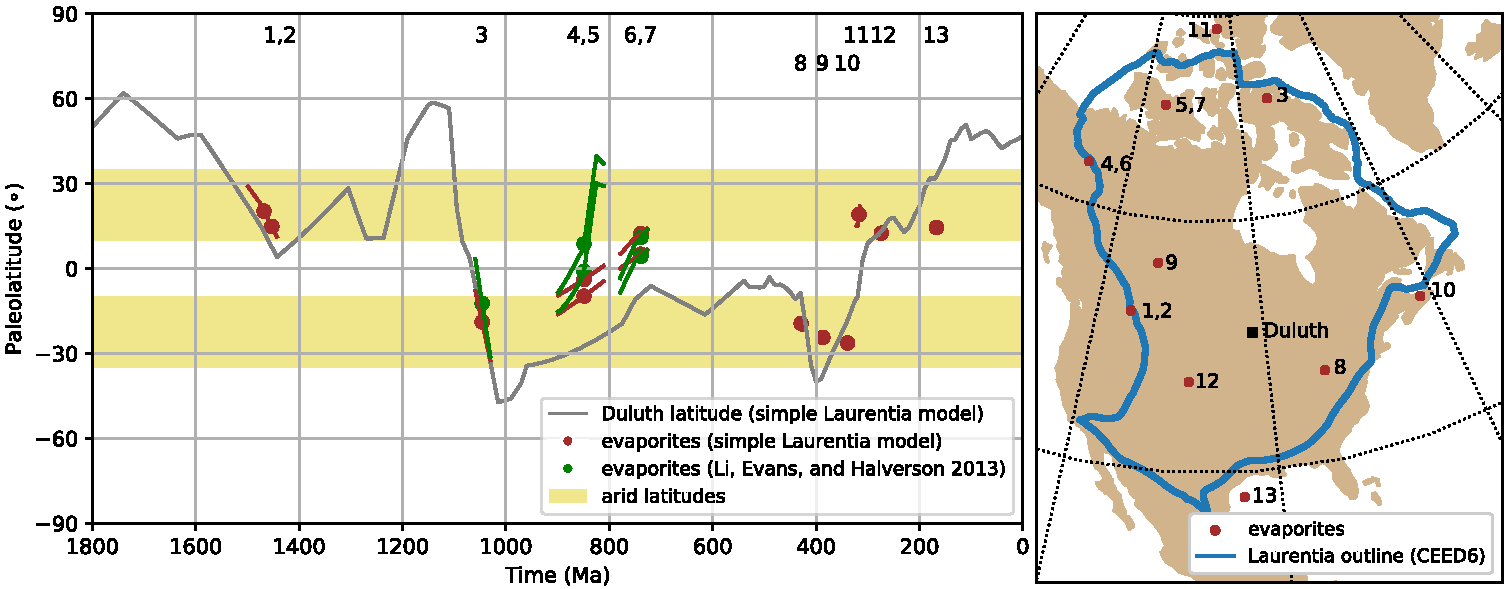
\includegraphics[width=7 in]{../Figures/Fig7_Laurentia_evaporite_figure.pdf}
\caption{\textbf{Paleolatitude of Laurentia evaporites.} Left panel: The paleolatitude of evaporite deposits as reconstructed by the simple Laurentia model shown in Fig. \ref{fig:Laurentia_paleolatitude} combined with the Phanerozoic model of \cite{Torsvik2017a} and as reconstructed by the model of \cite{Li2013a} for the Neoproterozoic. Proterozoic evaporite deposits in this panel are discussed in the text while Phanerozoic ones are taken from the compilation of \cite{Evans2006a}. The evaporite lines extend from the maximum to minimum age constraints with points at the preferred depositional age. The evaporite paleolatitude points are labeled with numbers that correspond to the numbers on the present-day location map in the right panel. These numbers correspond to: 1 -- Altyn Formation (Belt-Purcell Supergroup); 2: Wallace/Helena Formations -- Belt-Purcell Supergroup; 3 -- Iqqittuq Formation (Bylot Supergroup); 4 -- Ten Stone Formation (Mackenzie Mountains Supergroup); 5 -- Minto Inlet Formation (Shaler Supergroup); 6 -- Redstone River Formation (Mackenzie Mountains Supergroup); 7 -- Kilian Formation (Shaler Supergroup); 8 -- Silurian Michigan Basin ; 9 -- Devonian Western Canada; 10 -- Carboniferous Canadian Maritime; 11 -- Carboniferous Sverdrup; 12 -- Permian Midcontinental USA; 13 -- Jurassic Gulf of Mexico.}
\label{fig:Laurentia_evaporites}
\end{figure*}

Proterozoic evaporite deposits are documented within the following units that were deposited following the amalgamation of Laurentia (Fig. \ref{fig:Laurentia_evaporites}): 
\begin{itemize}
%\item The Stark Formation of the Slave Province contains displacive halite pseudomorphs throughout as well as massive breccias  interpreted to be evaporite-collapse breccias \citep{Pope2003a}. The formation is intruded by 1865 $\pm$ 15 Compton laccoliths  and is interpreted to have been deposited 
\item The Altyn Formation of the Belt-Purcell Supergroup contains pseudomorphs after gypsum crystals and anhydrite within shallow-water carbonates with relict gypsum and anhydrite preserved within secondary silica \citep{White1984a}. The correlative Prichard Formation is intruded by 1468.8 $\pm$ 2.5 Ma sills \citep{Sears1998a}. Halite molds and casts are present within mudstones of the overlying Grinell Formation \citep{Pratt2019a}. Higher in the Belt-Purcell Supergroup stratigraphy, within the Wallace Formation, there is stratiform scapolite --- a metamorphic mineral interpreted to have formed from a halite precursor within the Wallace Formation \citep{Hietanen1967a}. There are also halite and gypsum pseudomorphs within carbonate mudstones of the correlative to underlying Helena Formation \citep{Pratt2001a,Winston2007a}.  These deposits are older than the 1443 $\pm$ 7 Ma Purcell lavas and further constrained in age by a tuff with a U-Pb date of 1454 $\pm$ 9 Ma within the Helena Formation \citep{Evans2000c}. 
\item The Mesoproterozoic Iqqittuq Formation of the Borden basin (formerly part of the Society Cliffs Formation) contains bedded gypsum deposits (massive and laminated with beds that reach a thickness of 2.5 meters) and shale with halite casts \citep{Kah2001a}.  These deposits are bracketed between Re-Os dates of 1048 $\pm$ 12 Ma for an underlying shale and 1046 $\pm$ 16 Ma for an overlying shale \citep{Gibson2018a}.
\item The Tonian Ten Stone Formation of the Mackenzie Mountains Supergroup (formerly known as the Gypsum Formation) contains a $\sim$500 meter thick succession dominated by gypsum with minor anhydrite interpreted to have been deposited in a deep-water (below wave base) restricted marine basin \citep{Turner2016a}. These thick bedded sulfate deposits are older than cross-cutting 775.1 $\pm$ 0.5 Ma sills of the Gunbarrel large igneous province (U-Pb date from \citealp{Milton2017a}) and younger than ca. 1005 Ma detrital zircons \citep{Turner2016a}. The overlying Ram Head Formation has been correlated with the Bitter Springs Stage which is constrained between 811.5 $\pm$ 0.3 Ma and 788.7 $\pm$ 0.2 Ma \citep{Macdonald2010a, Swanson-Hysell2015a} suggesting that the evaporites are ca. 820 Ma \citep{Turner2016a}. These deposits are hypothesized to be correlative with sulfate evaporites within the Minto Inlet Formation of the Shaler Supergroup \citep{Jones2010a, Turner2016a}.
\item The Tonian Kilian Formation of the Shaler Supergroup contains nodules of gypsum and anhydrite interpreted to have been deposited in an intertidal to supratidal evaporitic mudflat environment \citep{Prince2014a}. The Kilian Formation is interpreted to post-date the Bitter Springs Stage and be correlative with the Redstone River Formation of the Coates Lake Group in the Mackenzie Mountains that contains bedded gypsum as well as gypsum-bearing siltstone \citep{Jefferson1989a, Jones2010a}. The Redstone River Formation is younger than the 777.7 $\pm$ 2.5 Ma volcanics and older than a 732.2 $\pm$ 4.7 Ma Re-Os date from the overlying Coppercap Formation \citep{Rooney2014a}. These units are also interpreted to be correlative with the Callison Lake Formation which contains pseudomorphs after gypsum and is constrained to have been deposited between Re-Os dates of 752.7 $\pm$ 5.5 Ma and 739.9 $\pm$ 6.5 Ma \citep{Strauss2015a}.
\end{itemize}

In Figure \ref{fig:Laurentia_evaporites}, the paleolatitude of these evaporite deposits are reconstructed using the simple Laurentia model developed in this work as well as with the \cite{Li2013a} model for the late Mesoproterozoic to Neoproterozoic. The position of major Phanerozoic evaporite basins of North America are also shown with their paleolatitude reconstructed with the paleogeographic model of \cite{Torsvik2017a}. These paleogeographic models reconstruct evaporite deposition to have been within 30\textdegree\ of the equator in both the Phanerozoic and Proterozoic. In the Tonian period, evaporite deposition may have occurred equatorward of 10\textdegree\ (Fig. \ref{fig:Laurentia_evaporites}). In interpreting these data, it is important to note that there is high evaporation in the subtropics and the tropics. Within the tropical rain belt (0 to $\sim$10\textdegree\ latitude) these high evaporation rates are typically overwhelmed by precipitation such that global zonal mean precipitation exceeds evaporation within $\sim$10\textdegree\ of the equator (within $\sim$8\textdegree$\;$ of the equator over land). Evaporation typically exceeding precipitation from those latitudes ($\sim$10 to 15\textdegree) towards higher ones with evaporation minus precipitation being at a maximum at $\sim$20-25\textdegree\ \citep{Park2021a}. However, continental interiors near the equator can also be arid due to regional precipitation patterns leading to aridity and the formation of evaporites. For example, Lake Magadi in Kenya at a latitude of 1.9\textdegree S is a saline lake where thick bedded evaporites have accumulated \citep{Eugster1980a}. Caution is therefore needed when interpreting paleolatitude from evaporites in terrestrial and intracratonic settings given that they could occur both in tropical and subtropical latitudes. Therefore low-latitude evaporites ca. 750 Ma could reflect increased aridity in the tropical interior of the Rodinia supercontinent. Overall, the paleomagnetic data as synthesized in the paleogeographic models are in agreement with the Laurentia evaporite record from the Mesoproterozoic to the Cenozoic (Fig. \ref{fig:Laurentia_evaporites}).

\subsection{Evaluating Laurentia's Proterozoic paleogeographic neighbors}

Many different paleogeographic connections between Laurentia and other Proterozoic cratons have been proposed and utilized in paleogeographic models both prior to and following the amalgamation of Laurentia's constituent Archean provinces. This section is not comprehensive in terms of proposed connections, but rather I seek to highlight and contextualize some of the more prominent and/or well-supported models. These connections are often discussed in the context of hypothesized supercontinents given the hypothesis that Laurentia was an important constituent of Nuna, following ca. 1.85 Ga Trans-Hudson orogenesis, and of Rodinia, following ca. 1.05 Ga Grenvillian orogenesis. 

\subsubsection{Paleogeographic connections prior to initial Laurentia assembly}

Within this volume, \cite{Salminen2021a} describe proposed Neoarchean to Paleoproterozoic groupings of Archean provinces (``supercratons'' in the terminology of \citealp{Bleeker2003a}) prior to Laurentia assembly. In particular, they discuss the hypothesis of Superia (named after the Superior province) wherein the Superior province of Laurentia is central to a group of Archean lithospheric blocks \citep{Bleeker2006a}, including the Kola and Karelia provinces of Baltica and the Wyoming province of Laurentia, that broke up prior to 2.0 Ga. This hypothesis was based on proposed shared connections in the source of mafic intrusive rocks from 2.45 to 2.11 Ga with Kola and Karelia on the southeastern margin of the Superior Province \citep{Davey2020a}. \cite{Salminen2021a}  argue that the originally proposed Superia fit is not consistent with Baltica paleomagnetic poles. Instead, they propose a Superia (II) fit where there is a connection between the blocks between 2.68 and 2.05 Ga with some internal rotations. Another proposed connection evaluated by \cite{Salminen2021a}, also based on the correlation of mafic dikes, is one between the Slave province of Laurentia and the Dharwar province of India \citep{French2010a} as part of Sclavia (named after the Slave province; \citealp{Bleeker2003a}). This Slave-Dharwar connection is found to be consistent with ca. 2.23 Ga and ca. 2.19 Ga pairs of paleomagnetic poles if modified into a Sclavia (II) orientation \citep{Salminen2021a}. These blocks would have had a distinct drift history from Superia for most of the Paleoproterozoic \citep{Salminen2021a}.

\begin{figure*}
\centering
\includegraphics[width=\textwidth]{../Figures/Fig8_Rodinia_Reconstruction.pdf}
\caption{\textbf{Paleogeographic reconstructions of Laurentia and other select conjugate Proterozoic continents leading up to Rodinia assembly in the late Mesoproterozoic and to its initial break-up in the Neoproterozoic}. The hypothesized connection between Siberia and Laurentia is implemented following \cite{Evans2016b} who interpret this relationship as persistent from 1.7 to 0.7 Ga. The reconstruction of North China to Laurentia following \cite{Ding2021a}. The reconstruction implements Kalahari and Amazonia cratons as conjugates with Laurentia in the Grenvillian orogeny \citep{Hoffman1991a}. The Australia-East Antarctica relationship with Laurentia follows \cite{Swanson-Hysell2012a} and is similar to the Neoproterozoic reconstruction between the continents of \cite{Li2011a} and implementing their relative rotation of North Australia relative to South and West Australia. This configuration back to ca. 1140 Ma is consistent with a comparison between the Laurentia poles of that age and the coeval Mt. Isa dikes pole from North Australia and with the Keweenawan Track if the the Nonesuch and Freda poles are interpreted to be ca. 1080 (consistent with chronostratigraphic constraints; \citealp{Slotznick2018b}) with further motion by ca. 1070 Ma. The time slices show the rapid motion of Laurentia implied by the paleomagnetic poles which is consistent with the timing of collisional orogenesis associated with the Grenvillian orogeny. The assembled Rodinia persisted until initial rifting ca. 775 Ma with episodic rifting continuing until ca. 530 Ma.}
\label{fig:Grenville_reconstructions}
\end{figure*}

\subsubsection{Amazonia}

In the central and southern Appalachians there are inliers of rocks that were metamorphosed during the Ottawan phase of the Grenvillian orogeny \citep{McLelland2013a}. On the basis of whole-rock Pb-isotope data, \cite{Loewy2003a} and \cite{Fisher2010a} proposed that these inliers are fragments of lithosphere of another continent that were transferred to Laurentia during the Grenvillian orogeny and left behind when the Iapetus Ocean formed. In particular, \cite{Fisher2010a} suggested that the Suns\'as orogen of Amazonia is the best match for southern and central Appalachian inliers. This positioning is consistent with a paleogeographic model wherein Amazonia is a major portion of the conjugate continental lithosphere that collided with Laurentia during Rodinia assembly (Fig. \ref{fig:Grenville_reconstructions}; \citealp{Hoffman1991a, Evans2013b, Cawood2017a}). While the lack of ca. 1100 to 1000 Ma poles from Amazonia precludes a robust paleomagnetic test, this scenario is consistent with the available late Mesoproterozoic poles from Amazonia (ca. 1200 Nova Floresta pole and ca. 1150 Fortuna Formation pole; \citealp{DAgrella-Filho2021a}) as shown in \cite{Evans2013b}. In this paleogeographic scenario, the basement inliers of the Appalachian Orogen in the Blue Ridge region are interpreted to be the leading edge of Amazonia with initial collision ca. 1080 Ma initiating the Ottawan phase of the Grenvillian orogeny (Fig. \ref{fig:tectonic_history}). Subsequent separation of Amazonia in the Neoproterozoic would have led to the formation of the Iapetus Ocean as Rodinia rifted apart. Departure of Amazonia potentially occurred as early as ca. 700 Ma in the Paleo-Iapetus Ocean model of \citet{Robert2020a} in conjunction with rifting in eastern Laurentia. A significantly later separation ca. 560 Ma would be predicted if Amazonia were further north (present-day coordinates) along Laurentia's margin given the lack of evidence of earlier rifting until after ca. 620 Ma north of the New York promontory \citep{Allen2010a}.

\subsubsection{Australia and East Antarctica}

It has long been argued that there are shared aspects of the geologic history between Australia, East Antarctica and Laurentia \citep{Moores1991a}. The extent of Antarctic lithosphere that was conjoined with Australia prior to the assembly of Gondwana is uncertain, but there are strong connections between the Gawler province of the South Australia craton and the Terre Ad\'elie province of Antarctica that is commonly interpreted to extended to the Miller ranges of the Trans-Antarctic Mountains as the Mawson craton \citep{Payne2009b}.  Separation between these Antarctic provinces and Australia was largely accomplished in the current Cenozoic Era with the opening of the Tasmanian seaway. Correlations with Laurentia have led to a number of distinct proposed reconstructions of Australia + East Antarctica along the western margin of Laurentia at different times in the Proterozoic.

Metamorphism ca. 1.6 Ga on the eastern margin of the North Australia craton associated with the Issan-Jana orogeny has been interpreted to be the  result of collisional orogenesis with the western Laurentia margin \citep{Nordsvan2018a, Pourteau2018a, Gibson2020a}. That Laurentia was the conjugate continent for this orogeny is argued to be supported by detrital zircon date spectra from the Georgetown Inlier of the eastern North Australia craton that have similarities with possible Laurentia sources \citep{Nordsvan2018a}. In the model of \cite{Nordsvan2018a}, the inlier is a continental ribbon that rifted from Laurentia ca. 1.68 Ga and was then caught up in ca. 1.60 Ga collision between the North Australia craton and northwestern Laurentia although others interpret it to be part of an extended Australian margin \citep{Gibson2020a}. The ca. 1.60 Ga Racklan-Forward orogeny in northwestern Laurentia records arc-continent collision that could have been followed by continent-continent collision between Laurentia and Australia \citep{Thorkelson2005a, Furlanetto2013a}. This timing of the conjoinment of the cratons would put Australia in a position that honors subsequent Mesoproterozoic correlations. Detrital zircons dates of ca. 1.61 to 1.50 Ga in the ca. 1.45 Ga lower Belt-Purcell supergroup of Laurentia are interpreted to have been sourced from the North Australia craton \citep{Jones2015a}. The U-Pb-Hf signatures of detrital zircons from ca. 1.45 to 1.30 Ga sedimentary rocks of Tasmania have also been interpreted to indicate a Laurentia source consistent with such a paleogeographic connection \citep{Mulder2015a}. Additionally, ca. 1.44 Ga granites in East Antarctica (recovered as glacial clasts and inferred from detrital zircons) have the same age and isotopic signatures as the distinctive `A-type' granites in Laurentia \citep{Goodge2008a}. The interpretation of \cite{Goodge2008a, Goodge2017a} is that there is an extension of the southwestern Laurentia A-type magmatic belt into Antarctica (that is currently overlain by the East Antarctic ice sheet). The correlation of the eastern North Australia craton with northwestern Laurentia and that of \textbf{s}outh\textbf{w}est Laurentia with \textbf{E}ast \textbf{A}n\textbf{t}arctica leads to the SWEAT fit proposed to have initiated in the Paleoproterozoic by \cite{Moores1991a}. Given that this tight-fit configuration likely was not sustained into the Neoproterozoic, as discussed below, researchers have taken to referring to this configuration as  the ``proto-SWEAT'' reconstruction \citep{Payne2009b, Kirscher2020a}. A comparison between paleomagnetic data from the ca. 1.32 Ga Derim Derim sills of the North Australia craton and the ca. 1.31 Ga Nain anorthosite of Laurentia are consistent with this SWEAT configuration leading to the interpretation that it persisted from 1.6 Ga to at least 1.3 Ga \citep{Kirscher2020a}. If the North Australian craton was continuous with South Australia, this interpretation would have the ca. 1.47 to 1.40 Ga Belt-Purcell basin be an intracontinental rift and makes it more difficult to explain the ca. 1.35 Ga East Kootenay orogeny on that margin. A paleomagnetic pole from the ca. 1.21 Ga Gnowangerup-Fraser dike swarm is argued to be inconsistent with a conjoined relationship between Australia and Laurentia ca. 1.2 Ga as it implies a high-latitude for Australia and distinct shape of the apparent polar wander path \citep{Pisarevsky2014a}. There is not a coeval pole from Laurentia for comparison ca. 1.21 Ga and data do indicate poleward motion for Laurentia between the ca. 1.24 and 1.18 Ga constraints. Nevertheless, comparison between latest Mesoproterozoic (ca. 1070 Ma) and Neoproterozoic (ca. 750 Ma) paleomagnetic poles from Australia and Laurentia are inconsistent with a configuration where Australia+East Antarctica are both tightly positioned against western Laurentia as they are in the proto-SWEAT fit. Rather, while these pole comparisons could be consistent with East Antarctica against southwestern Laurentia, they require the eastern Australian margin to be rotated further away from Laurentia as in Figure \ref{fig:Grenville_reconstructions}. There is a similarity between Australia's paleomagnetic pole database and that of Laurentia's in that both pole paths have a similar position between ca. 1070 Ma and ca. 770 Ma poles \citep{Swanson-Hysell2012a}. This similarity could support interpretations of a unified Rodinia containing both Australia and Laurentia throughout that time interval \citep{Swanson-Hysell2012a} that subsequently broke up ca. 650 Ma \citep{Li2011a}.

\subsubsection{Baltica}

Based on correlation of Archean provinces and Paleoproterozoic orogenic belts, \cite{Gower1990a} reconstructed Baltica to Laurentia in a position known as the NENA (northern Europe and North America) configuration. This configuration had originally been proposed by \citet{Patchett1978a} and \citet{Piper1980a} largely on the basis of paleomagnetic pole comparisons. This connection proposes a tight fit between present-day northern Norway and Russia's Kola Peninsula with eastern Greenland \citep{Gower1990a, Salminen2021b}. In this position, Baltica and Laurentia are hypothesized to share a long-lived accretionary margin wherein the Gothian orogen of Baltica (where accretionary orogenesis was active ca. 1.66 to 1.52 Ga; \citealp{Bergstrom2020a}) is a continuation of the Mazatzal-Labradorian orogenic belts of Laurentia \citep{Karlstrom2001a}. Baltica and Laurentia as conjoined cratons with a shared active margin features as a major component of Paleoproterozoic to Mesoproterozoic paleogeographic reconstructions \citep{Evans2011a, Zhang2012a, Elming2021a}. Rotating Baltica into the NENA connection position results in matched paleomagnetic pole pairs between ca. 1.78 to 1.26 Ga \citep{Buchan2000a, Evans2008a, Swanson-Hysell2021a} that could be extended to ca. 1.12 Ga if a virtual geomagnetic pole (that is a pole position calculated from paleomagnetic data of a single cooling unit) from the Salla dike of northeastern Finland is considered to be a representative paleomagnetic pole for Baltica \citep{Salminen2009b}. These data constrain the NENA connection to have been maintained until at least 1.26 Ga and perhaps until 1.12 Ga \citep{Salminen2021b}. 

Many paleogeographic models consider there to still have been close proximity between Baltica and Laurentia in the latest Mesoproterozoic into the Neoproterozoic. This continued connection has been hypothesized based on correlation of the Grenvillian orogeny with the Sveconorwegian orogeny of southwestern Baltica \citep{Gower1990b} as well as proposed similarities between the apparent polar wander path of Laurentia's Grenville loop and Baltica's Sveconorwegian loop that led reconstructions to be based on the alignment of these paths and the resulting position of Baltica relative to Laurentia \citep{Piper1980a,Pisarevsky2003a}. However, as geochronology has improved (e.g. \citealp{Gong2018b}), the ages of poles in the Sveconorwegian loop are now constrained to be younger than the Grenville loop poles falling in a gap in Laurentia's pole record \citep{Evans2015a,Fairchild2017a} which makes it more challenging to test proposed post-NENA configurations between the cratons.

In terms of the orogenic timing, the main phase of the Sveconorwegian orogeny from ca. 1.05 to 0.98 Ga corresponds temporally with the Grenvillian orogeny \citep{Stephens2020a}. There is currently an active debate in the literature whether the Sveconorwegian orogen is the result of collisional or accretionary orogenesis \citep{Stephens2020a}. \cite{Slagstad2019a} favor an accretionary orogeny and by contrasting this setting with the collisional orogenesis of the Grenvillian orogen argue that there should not be a link between Laurentia and Baltica ca. 1.0 Ga. However, in a recent critical review of the constraints, the high pressure nature of metamorphism and the cratonward propagation of orogenesis (in contrast to older accretionary orogenesis) led \cite{Stephens2020a} to favor the interpretation that the Sveconorwegian orogen is a record of prolonged continent-continent collision initiating ca. 1.06 Ga. In this model, Baltica could have been on the same plate as Laurentia during the rapid late Mesoporoterozoic motion leading up to collisional Grenvillian orogenesis and the associated assembly of Rodinia (Fig. \ref{fig:Grenville_reconstructions}).

Early Tonian intrusive granitoids and extrusive calc-alkaline volcanics in East Greenland and related Arctic terranes including northeast Svalbard, with ages between 975 to 915 Ma \citep{McClelland2019a}, are interpreted to have formed within a magmatic arc or in a syn-collisional setting \citep{Johansson1999a}. This magmatic activity is hypothesized to be the result of subduction and accretionary orogenesis termed the Valhalla orogeny \citep{Cawood2010a}. This geological evidence for an active margin in East Greenland in the earliest Neoproterozoic has motivated a tectonic model wherein Baltica rifted off East Greenland in the late Mesoproterozoic while staying proximal to Laurentia via a clockwise rotation that would have severed the NENA connection \citep{Cawood2010a}. Such a clockwise rotation of Baltica relative to Laurentia from the earlier Paleoproterozoic-Mesoproterozoic NENA configuration with a shared Labradorian to Gothian orogenic belt to one where the Sveconorwegian orogen is close to the Grenvillian orogen in Labrador (northeast Canada) is implemented in many paleogeographic models (e.g. \citealp{Evans2009a} and as shown in Fig. \ref{fig:Grenville_reconstructions}). This position relative to Laurentia results in a joint Laurentia-Baltica APWP with large oscillations implied by Baltica poles. These oscillations would imply that following the Grenville loop, Laurentia moved northward across the equator and then back south to a similar Grenville loop position prior to the ca. 780 Ma Laurentia poles \citep{Evans2015a,Fairchild2017a}.  A challenge with this model in terms of regional tectonics, is that it is unclear what conjugate lithosphere rifted from East Greenland leading to the thick sedimentary succession interpreted to have been deposited on a thermally-subsiding passive margin from ca. 850 Ma into the Cryogenian (Fig. \ref{fig:tectonic_history}; \citealp{Maloof2006a}). \cite{Malone2014a} interpreted this Neoproterozoic basin development along the East Greenland margin to have been the result of extension in a back-arc setting. 

Magmatism ca. 615 Ma in both Laurentia and Baltica (in the relative configuration shown in Figure \ref{fig:Grenville_reconstructions}) is interpreted to be associated with the plume-related Central Iapetus Magmatic Province (CIMP; \citealp{Tegner2019a}). This ca. 615 to 590 Ma magmatism is hypothesized to have initiated the breakup between Baltica and Laurentia that led to the opening of the Iapetus Ocean (Figs. \ref{fig:tectonic_history} and \ref{fig:Grenville_reconstructions}; \citealp{Cawood2001a, Tegner2019a}). The cratons would once again be conjoined ca. 430 Ma during their collision that led to the Caledonian orogeny resulting in a continent that is referred to as Laurussia \citep{Torsvik2017a}.

\subsubsection{Kalahari}

High-quality paleomagnetic poles constrain the coeval ca. 1109 Ma Umkondo large igneous province of the Kalahari craton and the early flood basalts of the Midcontinent Rift of Laurentia to have been separated by more than 50\textdegree\ of latitude at the time they were emplaced. These poles reconstruct the craton margins as having been separated by more than 30\textdegree\ of latitude \citep{Swanson-Hysell2015a}. These data make it difficult to envision a shared origin of magmatism and pose a challenge to approaches that seek to reconstruct paleogeography on the basis on ages of LIPs alone. However, with the subsequent rapid motion of Laurentia to low latitudes (Figs. \ref{fig:Laurentia_paleolatitude} and \ref{fig:Grenville_reconstructions}), it is possible that the Kalahari was a conjugate craton to the (south)eastern margin of Laurentia during the time of the Grenvillian orogeny. This conjugate relationship based on the interpretation that the Namaqua-Natal belt in southern Kalahari records late Mesoproterozoic collisional orogenesis was proposed in \cite{Hoffman1991a} and is implemented in most reconstructions of Rodinia (e.g. \citealp{Li2008a}). Whether the Grenvillian margin of Laurentia and the Namaqua-Natal belt of Kalahari faced one another and could have been conjugates can be evaluated by paired paleomagnetic and geochronologic data sets from the Umkondo LIP and the Midcontinent Rift. The preferred interpretation of \cite{Swanson-Hysell2015a} and \cite{Kasbohm2015a} is that sites with northerly declinations from the Umkondo Province correspond to the reversed polarity directions from the early magmatic stage in the Midcontinent Rift (e.g. \citealp{Swanson-Hysell2014a}) such that Namaqua-Natal margin faced the Grenvillian margin of Laurentia (Fig. \ref{fig:Grenville_reconstructions}). The late Mesoproterozoic apparent polar wander paths for Laurentia and Kalahari are consistent with them becoming conjoined as in Figure \ref{fig:Grenville_reconstructions} \citep{Swanson-Hysell2015a}. The record of the Namaqua belt wherein there is granitoid plutonism and arc accretion up to ca. 1090 followed by peak granulite metamorphism ca. 1065 to 1045 Ma \citep{Diener2013a, Spencer2015a} is consistent with a scenario wherein Kalahari was on the upper plate that collided with Laurentia at the time of the Ottawan phase of Grenvillian orogenesis following subduction of oceanic lithosphere associated with an intervening ocean. If they indeed became conjoined in Rodinia as in Figure \ref{fig:Grenville_reconstructions}, the separation of Kalahari from Laurentia may have initiated ca. 795 Ma heralded by the emplacement of the Gannakouriep diabase dike swarm \citep{Rioux2010a, DeKock2021a} and volcanic rocks in southeastern Laurentia (e.g., the ca. 750 Ma Mount Rogers volcanics and associated rift-related sediments \cite{Aleinikoff1995a, MacLennan2020a}). A ca. 750 Ma volcano-sedimentary sequence in northwest Kalahari is interpreted to be rift-related \citep{Borg2003a}  and could be correlative with the Mount Rogers Formation. This late Tonian timing for separation could be consistent with a position along the southeastern Laurentia margin, although subsequent Ediacaran rifting and Cambrian thermal subsidence in the region would need to be attributed to the rifting of microcontinents such as Arequipa and Cuyania \citep{Escayola2011a, Martin2019a}.

\subsubsection{North China}

The latest Mesoproterozoic to earliest Neoproterozoic pole path of the North China craton includes a swath of paleomagnetic poles with a similar arc length to the Keweenawan Track to Grenville Loop of Laurentia's APWP \citep{Zhao2019a, Ding2021a, Zhang2021a}. While the chronostratigraphic age constraints on these North China poles are much looser than those from Laurentia, \cite{Zhao2019a} proposed that the North China poles can be aligned with the Keweenawan Track to reconstruct North China as being conjoined to the northwestern margin of Laurentia from prior to ca. 1110 Ma into the early Neoproterozoic. In this model, North China would have been at polar latitudes ca. 1110 Ma and moved rapidly with Laurentia as it transited towards the equator. A challenge with interpreting these North China poles as primary is that they include data from limestones that would reconstruct them to have been deposited at very high latitude ($>$80\textdegree\ for the limestones of the lower member of the Nanfen Formation). Such high-latitude limestones would require non-uniformitarian depositional conditions for carbonate precipitation which is more dominant in low latitudes due to the temperature dependence of carbonate saturation. As additional support for a North China--Laurentia connection, \cite{Zhao2019a} pointed to similarities in the detrital zircon age spectra between early Neoproterozoic sediments in NW Laurentia and North China basins as supporting this reconstruction. In particular, sediment transport from Laurentia could provide a source for ca. 1.18 Ga zircons (from the Shawinigan orogen) and ca. 1.08 Ga zircons (from the Grenville orogen). In the Laurentia basins, ca. 1.6 Ga zircons without a clear Laurentia source could be sourced from North China craton granites (e.g. \citealp{Wang2020a}). If North China was in this position, the timing of its arrival adjacent to Laurentia is unclear. The ca. 1220 Ma dikes pole of the North China craton is not coincident with the 1237 $\pm$ 5 Ma Sudbury dikes pole in this reconstructed position leading \cite{Zhao2019a} and \cite{Zhang2021a} to suggest that North China arrived on the Laurentian margin between ca. 1220 and 1110 Ma although they note a lack of evidence for known North China orogenesis at this time. Laurentia's pole path has a gap from the 1237 $\pm$ 5 Ma Sudbury pole to the 1184 $\pm$ 5 Ma Narssaq Gabbro and Hvidaal dike poles during which it ascends to the Logan Loop (Figs. \ref{fig:Laurentia_poles} and \ref{fig:Laurentia_paleolatitude}). In its reconstructed position, the ca. 1220 Ma North China pole is close to this gap such that it is possible that the APWPs are consistent and that North China arrived on the northwestern Laurentia margin prior to 1220 Ma. In terms of departing from this position, one possibility is that its departure is associated with latest Neoproterozoic extension in northwestern Laurentia.

\subsubsection{Siberia}

Southern Siberia and northern Laurentia have been proposed to be connected on the basis of a similar history of Paleoproterozoic collision \citep{Rainbird1998a}, matches in the age of mafic intrusives rocks interpreted as shared large igneous provinces from the Paleoproterozoic to the Neoproterozoic \citep{Ernst2016a}, and comparisons of paleomagnetic poles \citep{Evans2011a, Evans2016b}. U-Pb dates from mafic intrusive rocks are interpreted by \cite{Ernst2016a} as resulting from shared large igneous provinces between southern Siberia and northern Laurentia from the time of Laurentia's amalgamation ca. 1.8 Ga all the way up to the time of the ca. 720 Ma Franklin large igneous province (LIP). For example, mafic intrusions and lavas that are grouped as the Irkutsk LIP in Siberia have been dated in Siberia to be similar in age to dates developed from the Franklin LIP \citep{Denyszyn2009a, Ernst2016a}. Comparisons of paleomagnetic poles between Laurentia and Siberia support this tight and internally stable fit between southern Siberia and northern Laurentia from ca. 1.64 to at least ca. 0.76 Ga  \citep{Evans2016b}. Overlap in Laurentia and Siberia pole positions with such a reconstruction are achieved in the Statherian Period of the Paleoproterozoic (the ca. 1.64 Ga Nersa complex of Siberia compared to the Melville Bugt dikes of Laurentia), the Calymmian Period of the Mesoproterozoic (the ca. 1.50 Ga Anabar intrusions with the ca. 1.48 Ga St. Francois Mountains igneous province of Laurentia), the Stentian Period of the Mesoproterozoic (a number of roughly chronostratigraphically constrained Siberia poles with the 1.11 to 1.08 Ga Keweenawan Track of Laurentia) and the Tonian Period of the Neoproterozoic (the ca. 758 Kitoi pole of Siberia with Tonian Laurentia poles).  The correlation of the Malgina pole of Siberia with the Keweenawan Track gains additional support in that it correlates the normal-polarity Maya superchron \citep{Gallet2012a} with the Portage Lake normal-polarity zone \citep{Swanson-Hysell2019a} that is interpreted as a normal-polarity superchron (termed the Keweenawan Normal Superchron in \citealp{Driscoll2016a}). This correlation both works with the tight fit and resolves hemispheric ambiguity to put both cratons together in the northern hemisphere ca. 1100 Ma (Fig. \ref{fig:Grenville_reconstructions}). Connections between Archean provinces may have also existed prior to Laurentia assembly such as the hypothesized connection between the Slave Province and the Tungus Province of Siberia which has the Thelon orogen correlated to Paleoproterozoic orogenesis in the Akitkan fold belt \citep{Condie1994a, Rainbird1998a, Evans2011a}.

The interpretation that the Franklin LIP is recorded in both Laurentia and Siberia constrains the break-up between the continents to post-date 720 Ma. While there could have been some extension in the Tonian Period and at the time of the Franklin emplacement, the record of northern Laurentia subsidence indicates Ediacaran to early Cambrian extensional tectonism (e.g. \citealp{Strauss2019a}). Therefore, it might not have been until the late Ediacaran Period that the long-term Proterozoic connection between the cratons ended.

\subsection{The record implies plate tectonics throughout the Proterozoic}
\label{sec:plate_tectonics}

\begin{figure*}
\centering
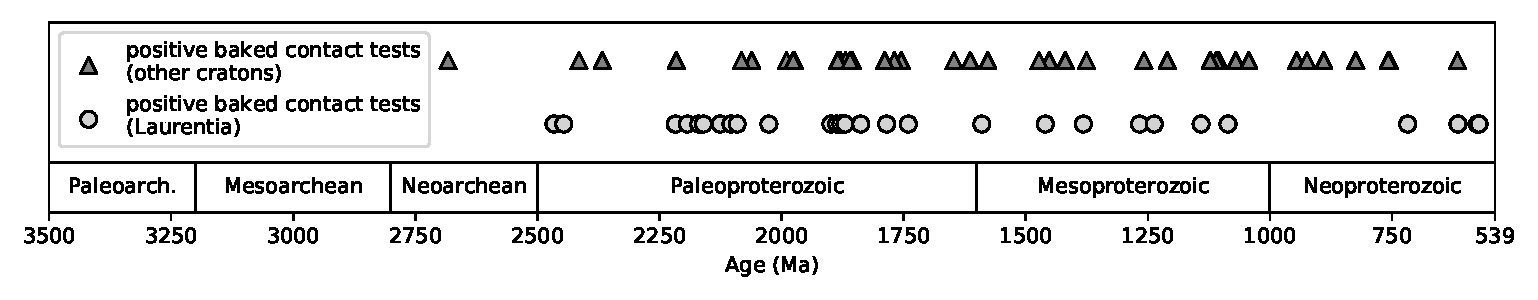
\includegraphics[width=\textwidth]{../Figures/Fig9_baked_contact_timeline_all.pdf}
\caption{\textbf{Paleomagnetic poles with positive baked contact tests from Laurentia and other cratons}. This timeline shows the age of paleomagnetic poles with positive baked contact tests within the Nordic Paleogeography Workshop compilation \citep{Evans2021a}. Positive baked contact tests require the presence of an appreciable geomagnetic field. In turn, the presence of geomagnetic field requires heat flow across the core mantle boundary that is maintained by plate tectonics, but that would be stifled by a stagnant lid.}
\label{fig:baked_contact}
\end{figure*}

Even without considering other continents, there is strong evidence both in Laurentia's geological and paleomagnetic record for differential plate tectonic motion between 2.2 and 1.8 Ga. The continued history of accretionary orogenesis and the evaluation of Laurentia's pole path in comparison to other continents from 1.8 Ga onward supports the continual operation of plate tectonics throughout the rest of the Proterozoic and Phanerozoic as well. While this evidence fits with the majority of interpretations of the timing of initiation of modern-style plate tectonics (see summary in \citealp{Korenaga2013a}), there continue to be proponents of a stagnant lid throughout the Mesoproterozoic Era (1.6 to 1.0 Ga) and into the Neoproterozoic  with plate tectonics not initiating until ca. 0.8 Ga \citep{Hamilton2011a, Stern2018a}. These arguments rest on the relative lack of Proterozoic low-temperature high-pressure metamorphic rocks such as blueschists that form in subduction zones \citep{Stern2013a}. Alternative interpretations for the lack of blueschists in the Proterozoic call upon both their low preservation potential or secular changes in mantle chemistry and/or temperature \citep{Brown2019a}. \cite{Palin2015a} proposed that such a shift in metamorphic regime is the predicted result of secular evolution of mantle chemistry and changing MgO composition of oceanic crust rather than a harbinger of the onset of plate tectonics. An alternative hypothesis is that earlier in the Proterozoic slab breakoff occurred at shallower depths limiting the formation and preservation of low-temperature/high-pressure metamorphic rocks \citep{Brown2019a}. In this model, secular mantle cooling led to increasingly strong lithosphere that enabled deeper continental subduction and slab breakoff depths. While the secular change in the abundance of low-temperature/high-pressure metamorphic rocks is intriguing, to argue that there was not differential plate tectonic motion in the Paleoproterozoic and Mesoproterozoic is to ignore a vast breadth and depth of geological and paleomagnetic data. From a paleomagnetic perspective, there is strong support for independent and differential motion between the Slave and Superior provinces from 2.2 to 1.8 Ga from as is illustrated in Figure \ref{fig:Superior_Slave_recons}. From a geological perspective, the Trans-Hudson orogenic interval, the Grenville orogenic interval, and the Appalachian orogenic interval are all well-explained with a mobilistic interpretation that includes phases of accretionary orogenesis followed by collisional orogenesis (Fig. \ref{fig:tectonic_history}). One could counter that this perspective results from a plate-tectonic-centric viewpoint that lacks creativity to see the record as resulting from other processes than modern-style plate tectonics. However, in addition to the broad geological record showing an amalgamation of terranes as would be expected to arise through plate tectonics, there are also Proterozoic obducted ophiolites that are well-explained through accretionary plate tectonics as well as eclogites such as those preserved in the Trans-Hudson orogen \citep{Weller2017a}. These eclogites preserve evidence for high-pressure/low-temperature metamorphic conditions ca. 1.8 Ga. Similar to the Himalayan orogen, these rocks are interpreted to be the result of deep subduction and exhumation of continental crust during convergent tectonics \citep{Weller2017a}. Outside of Laurentia, there are examples of Paleoproterozoic eclogites with geochemical affinity to oceanic crust such as that documented in the ca. 1.9 Ga Ubendian belt of the Congo craton \citep{Boniface2012a}. Mesoproterozoic ophiolites were also obducted to Laurentia such as the Pyrites ophiolite complex within the Shawinigan orogen and the Coal Creek Domain of the Llano uplift \citep{Chiarenzelli2011a, McLelland2013a}.

Another perspective on Proterozoic tectonics is that the record is one of intermittent subduction \citep{Silver2008a, ONeill2013a}. In such a model, there are extended intervals with a stagnant lid alternating with intervals of differential plate motion. In particular, it has been argued that the Mesoproterozoic Era was an interval when Earth was in a stagnant regime without mobile plate tectonics \citep{Silver2008a, ONeill2013a}. The long-lived accretionary history of Laurentia following the amalgamation of the Archean provinces is difficult to reconcile with such an interpretation (Figs. \ref{fig:Laurentia_map} and \ref{fig:tectonic_history}). The record of paleomagnetic poles also show that there was progressive motion of Laurentia through the Proterozoic (Figs. \ref{fig:Laurentia_paleolatitude} and \ref{fig:Laurentia_reconstructions}). Using data from Laurentia alone, however, it is difficult to ascertain whether this motion is due to plate tectonic motion or rotation of the entire solid Earth through true polar wander. True polar wander can lead to a changing position relative to the spin axis even with a stagnant lid. One interval when the Laurentian paleomagnetic record demands that some of the motion is through differential plate tectonics is in the latest Mesoproterozoic. At that time, the pole path is very well-resolved with many high-quality paleomagnetic poles between 1110 and 1070 Ma (Table 2; \ref{fig:Laurentia_poles}). The progression of the poles requires rotation about an Euler pole that is distinct from a great circle path which would result if the motion were solely due to true polar wander \citep{Swanson-Hysell2019a}. These poles constrain rapid motion of Laurentia leading up to collisional orogenesis associated with the Grenvillian orogeny, as illustrated in Figure \ref{fig:Grenville_reconstructions}. These data provide strong evidence for differential plate motion at the time and are inconsistent with a stagnant lid. Rather, the orogenic interval within the Mesoproterozoic bears similarity with that of the Paleozoic (0.54 to 0.25 Ga) and reveals Laurentia to have been a central player in amalgamation of continents associated with the supercontinents Rodinia and Pangea.

An additional constraint supporting ongoing plate tectonics throughout the Proterozoic comes from paleomagnetic evidence of a sustained geomagnetic field. In a prolonged stagnant lid regime, there would not be sufficient heat flow across the core-mantle boundary to sustain a geodynamo \citep{Nimmo2000a, Buffett2000b}. One way to get insight into the ancient geomagnetic field is through paleointensity experiments on igneous rocks that enable estimates of ancient field strength to be developed.  Paleointensity data developed from units that are also included within the Laurentia paleomagnetic poles database indicate a significant geomagnetic field in the Neoarchean \citep{Selkin2000a} through to the Mesoproterozoic \citep{Macouin2006a, Sprain2018a}. However, paleointensity experiments are challenging and prone to failure due to alteration during laboratory heating or non-ideal rock magnetic behavior. As a result, it is significantly more challenging to develop reliable paleointensity data than to develop the reliable paleodirectional data used to calculate paleomagnetic poles. Therefore, the paleointensity database is sparser than the compilation of reliable paleomagnetic poles. Paleodirectional data themselves can given insight into the presence of a significant geomagnetic field --- particularly those with positive baked contact tests (Fig. \ref{fig:baked_contact}). Baked contact tests indicate that, at the time of dike emplacement, there was an appreciable field such that both the cooling magma and the heated country rock in the vicinity of a dike were able to acquire a primary coherent magnetization direction. Additionally, since paleomagnetic poles are typically developed from many individual cooling units across a region, the similarity of the directions across an igneous province indicates that the magnetizations were dominantly acquired from the geomagnetic field rather than being influenced by local variable crustal magnetizations.  Therefore, the record of abundant positive baked contact tests and coherent paleomagnetic poles (Fig. \ref{fig:baked_contact}; Table 2) supports the persistence of a geomagnetic field through the Paleoproterozoic and Mesoproterozoic which implies active plate tectonics that enabled sufficient core-mantle boundary heat flow to power the geodynamo.

\subsection{Conclusion}

The paleogeographic record of Laurentia is rich in constraints through the Precambrian both in terms of the geological and geochronological data on tectonism and the record of paleomagnetic poles. Data from the Slave and Superior provinces of Laurentia provide what is arguably the strongest evidence of differential plate tectonics in the Rhyacian and Orosirian Periods of the Paleoproterozoic Era (2.3 to 1.8 Ga) leading up to the collision of these microcontinents during the Trans-Hudson orogeny. The collisions of these and other Archean provinces led to the formation of the core of Laurentia. Subsequent crustal growth occurred through multiple intervals of accretionary orogenesis through the late Paleoproterozoic and Mesoproterozoic until the continent-continent collision of the Grenvillian orogeny that was ongoing at the Mesoproterozoic-Neoproterozoic boundary (1.0 Ga). The lead-up to this orogeny was associated with rapid plate motion of Laurentia from high latitudes towards the equator recorded by the Logan Loop and Keweenawan Track of paleomagnetic poles. Following a return to high latitudes, as constrained by paleomagnetic poles of the Grenville Loop, Laurentia straddled the equator at the time of Cryogenian Snowball Earth glaciation as part of the Rodinia supercontinent. Rifting and passive margin development then isolated Laurentia in late Ediacaran period and into the early Paleozoic Era. Subsequent accretionary and collisional orogenesis occurred associated with the Appalachian orogenic interval with Laurentia first colliding with Avalonia-Baltica to become Laurussia and Laurussia then uniting with Gondwana to form the supercontinent Pangea. While the details of the conjugate continents to Laurentia are better reconstructed for this last Wilson cycle, the broad features of the Trans-Hudson, Grenvillian and Appalachian orogenic intervals bear similarities. In each case, accretionary collision of arc terranes was followed by continent-continent collision. The major difference is that the collisions of the Grenvillian and Appalachian orogenic intervals resulted in relatively minor growth of Laurentia compared to the Trans-Hudson orogeny. This difference is the result of break-up following the Grenvillian and Appalachian orogenic intervals having occurred along the same margin as collision while the major orogens of the Trans-Hudson orogenic interval have remained sutured. As a result, Laurentia has been a formidable continent for the past 1.8 billion years. As can be seen in the Chapters on Archean paleogeography \citep{Salminen2021b}, Nuna \citep{Elming2021a}, and Rodinia \citep{Evans2021b}, the constraints from Laurentia are at the center of paleogeographic models through the Precambrian and will continue to be as the next generation of paleogeographic models are developed.

%%%%%%%%%%%% Supplementary Methods %%%%%%%%%%%%
%\footnotesize
%\section*{Methods}

%%%%%%%%%%%%% Acknowledgements %%%%%%%%%%%%%
\footnotesize
\subsection*{Acknowledgements}
This work was supported by NSF CAREER Grant EAR-1847277. The manuscript benefited from reviews from Athena Eyster, David Evans, and Lauri Pesonen as well as discussions and manuscript feedback from Francis Macdonald, Yuem Park, Toby Rivers, Sarah Slotznick and Justin Strauss. Bruce Buffett provided insights on the implications of a stagnant lid regime on the generation of the geomagnetic field. Many participants in the Nordic Paleomagnetism Workshop have contributed to the compilation and evaluation of the pole list utilized herein. Particular acknowledgement goes to David Evans for maintaining and distributing the compiled pole lists. GPlates, and in particular the pyGPlates API, was utilized in this work \citep{Muller2018b}. Figures were made using Matplotlib \citep{Hunter2007a} in conjunction with cartopy \citep{Met-Office2010a} and pmagpy \citep{Tauxe2016a} within an interactive Python environment \citep{Perez2007a}. The chapter text as well as code, data, and reconstructions used in this paper are openly available and licensed for any form of reuse with attribution (CC BY 4.0) in this repository: \url{https://github.com/Swanson-Hysell-Group/Laurentia_Paleogeography}.

\printendnotes

\subsection*{Glossary}
\noindent\textbf{accretionary orogeny } Lithospheric deformation associated with the subduction of oceanic lithosphere and the addition of material from the downgoing plate such as island arcs.

\noindent\textbf{allochthonous } An adjective denoting that a rock or terrane originated in a position at significant distance from the lithospheric block where it currently resides.

\noindent\textbf{Archean } A geologic eon spanning from 4,000 to 2,500 million years ago (4 to 2.5 Ga).

\noindent\textbf{Archean province } A contiguous area of Archean continental lithosphere typically surrounded by Proterozoic orogens inferred to be suture zones (e.g. Superior province).

\noindent\textbf{Canadian shield } The large area of Canada with exposed Precambrian rock, or rock covered by thin soil, that is well-exposed due to Pleistocene glaciation erosion.

\noindent\textbf{collisional orogeny } Lithospheric deformation resulting from the collision of two significant provinces of continental lithosphere.

\noindent\textbf{conjugate } Adjective referring to continents or continental margins that were previously conjoined.

\noindent\textbf{craton } The stable and relatively immobile continental lithosphere in the interior of continents. In this chapter, craton is predominantly used in reference to Laurentia which formed through the collision of Archean provinces and grew further through subsequent accretionary and collisional orogenesis. Note that in other usages the term can be focused on stable Archean lithosphere such as the individual Archean provinces of Laurentia.

\noindent\textbf{Cryogenian Period } The geologic period that lasted from ca. 717 to 635 million years ago during which time there were two global glaciations. The start of the period is provisionally defined as the first evidence of low-latitude glaciation. It is the second geologic period of the Neoproterozoic Era being preceded by the Tonian Period and followed by the Ediacaran Period.

\noindent\textbf{Ediacaran Period } The third geologic period of the Neoproterozoic Era from ca. 635 to 539 Ma million years ago. It is the final period of the Proterozoic Eon and is followed by the Cambrian Period.

\noindent\textbf{Elzevirian orogen } The orogen resulting from the Mesoproterozoic Elzevirian orogeny when there was accretion of arc terranes to eastern Laurentia.

\noindent\textbf{evaporite } A chemical sedimentary deposit consisting of minerals that crystallize from water that supersaturated in salts due to evaporation.

\noindent\textbf{Ga } Giga-annum, one billion (10$^9$) years. This term is used as an abbreviation for ``billions of years before present.''

\noindent\textbf{geocentric axial dipole hypothesis } The hypothesis that when it is time-averaged, Earth's magnetic field is dominantly a dipole aligned with the spin axis. 

\noindent\textbf{geodynamo } The mechanism whereby convective flow in Earth's fluid outer core generates Earth's magnetic field.

\noindent\textbf{Granite-rhyolite province } A geologic province that comprises widespread Mesoproterozoic rhyolite and granite extending from Labrador, Canada to west Texas, USA.

\noindent\textbf{Grenville orogen } An orogen resulting from the collision Grenvillian orogeny between Laurentia and conjugate continent(s) near the end of the Mesoproterozoic.

\noindent\textbf{Hadley cell } Large-scale atmospheric circulation where air rises near the equator, flows poleward, and descends in the subtropics. This circulation drives convective tropical precipitation and the dry downwelling air leads to aridity in the subtropics.

\noindent\textbf{Hearne province } An Archean province of Laurentia extending from southern Alberta, Canada to Hudson Bay. It is framed by the Rae province to the northwest and the Trans-Hudson orogen to the southeast. It is also referred to as the Hearne craton.

\noindent\textbf{hematite } An iron oxide mineral with a formula of Fe\textsubscript{2}O\textsubscript{3} that commonly holds magnetization in geologic materials, particularly oxidized sedimentary rocks.

\noindent\textbf{juvenile } An adjective referring to rocks formed from melt recently extracted from the mantle.

\noindent\textbf{Laurentia } The Precambrian cratonic core of the North America continent and Greenland that formed through the amalgamation of Archean provinces in the Paleoproterozoic and subsequent accretion.

\noindent\textbf{large igneous province (LIP) } A region of voluminous and rapidly emplaced volcanics and intrusions that are typically of mafic composition. These provinces are often interpreted to be due to decompression melting of an upwelling mantle plume.

\noindent\textbf{lithosphere } The rigid outermost layer of the Earth that is broken into tectonic plates and responds to the emplacement of a load by flexural bending.

\noindent\textbf{Ma } Mega-annum, one million (10$^6$) years. This term is used as an abbreviation for ``millions of years before present.''

\noindent\textbf{Manikewan Ocean } An ocean basin interpreted to have existed between the  Slave+Rae+Hearne+North Atlantic provinces and Superior province that closed leading up to the Trans-Hudson orogeny.

\noindent\textbf{Mazatzal orogen } An orogen resulting from latest Paleoproterozoic accretion of volcanic arc and back-arc terranes with southern Laurentia.

\noindent\textbf{Medicine Hat province } An Archean province of Laurentia extending from northern Montana, USA into southern Alberta and Saskatchewan, Canada. It is framed by a suture with the Hearne province to the north, the Trans-Hudson orogen to the east, and the Great Falls tectonic zone to the south. It is also referred to as the Medicine Hat block.

\noindent\textbf{Mesoproterozoic } A geologic era spanning from 1,600 to 1,000 million years ago.

\noindent\textbf{Meta Incognita province } A province of Archean basement rocks that comprises most of southern Baffin Island. It is also referred to as the Meta Incognita microcontinent.

\noindent\textbf{Midcontinent Rift } A major Mesoproterozoic intracratonic rift where there was co-location of large igneous province magmatism and extension in Laurentia's interior centered on the Lake Superior region.

\noindent\textbf{monazite } A phosphate mineral (Ce,La,Nd,Th)(PO\textsubscript{4},SiO\textsubscript{4}) found as an accessory phase in metamorphic rocks that can be targeted by U-Pb geochronology to date metamorphic events.

\noindent\textbf{Nagssugtoqidian orogen } An orogen resulting from the Paleoproterozoic collision between the Rae and North Atlantic provinces.

\noindent\textbf{Neoproterozoic } A geologic era spanning from 1,000 to 539 million years ago.

\noindent\textbf{North Atlantic province } An Archean province of Laurentia in southernmost Greenland and northeastern Labrador, Canada. It is also referred to as the North Atlantic craton.

\noindent\textbf{Nuna } A hypothesized supercontinent interpreted to have formed late in the Paleoproterozoic era and to have broken apart during the Mesoproterozoic.

\noindent\textbf{ophiolite } Oceanic lithosphere that as been accreted onto continental lithosphere.

\noindent\textbf{orogen } A region of lithosphere that has undergone deformation during a mountain-building event (an \textbf{orogeny}).

\noindent\textbf{paleolatitude } The past latitude of a given point on Earth's surface at a given time typically calculated from paleomagnetic data using the geocentric axial dipole hypothesis.

\noindent\textbf{paleomagnetic pole } A calculated position from paleomagnetic data that is interpreted to correspond to the ancient position of Earth's spin axis (the north pole) through application of the geocentric axial dipole hypothesis. The uncertainty on the pole position is given as a circle with a radius of a given angle ($A_{95}$).

\noindent\textbf{Paleoproterozoic } A geologic era spanning from 2,500 to 1,600 million years ago.

\noindent\textbf{Penokean orogen } An orogen resulting from Paleoproterozoic accretion of an oceanic arc and the Marshfield terrane continental block along the southern margin of the Superior province.

\noindent\textbf{Phanerozoic } A geologic eon spanning from 539 million years ago to the present day.

\noindent\textbf{Picuris orogen } An orogen resulting from a Mesoproterozoic orogeny interpreted from metamorphic rocks with Mesoproterozoic-aged protoliths in northern New Mexico, USA.

\noindent\textbf{plate tectonics } A process where the lithosphere is in distinct pieces that move relative to one another. 

\noindent\textbf{Precambrian } A commonly used informal term to refer to geologic time prior to the Cambrian Period that started 539 million years ago.

\noindent\textbf{Proterozoic } A geologic eon spanning from 2,500 to 539 million years ago.

\noindent\textbf{province } A spatial entity with a shared geologic history. The term is used in this chapter to refer to Archean provinces that moved as independent cratonic blocks prior to Laurentia's amalgmation (e.g. the Superior province). It is also used to refer to zones of crustal growth associated with orogens and the products of contemporaneous magmatic activity (large igneous provinces).

\noindent\textbf{Rae province } An Archean province of Laurentia extending from the region of Lake Athabasca northeast to northern Baffin Island in arctic Canada. It is framed by the Thelon orogen to the west, the Taltson orogen to the southwest and the Hearne province to the east. It is also referred to as the Rae craton.

\noindent\textbf{Rodinia } A hypothesized supercontinent interpreted to have formed late in the Mesoproterozoic era at the time of the Grenvillian orogeny and to have broken apart during the Neoproterozoic.

\noindent\textbf{Slave province } An Archean province of Laurentia extending to the north from the region of Great Slave Lake in northern Canada. It is framed by the Thelon orogen to the east and the Great Bear Arc to the west. It is also referred to as the Slave craton.

\noindent\textbf{Shawinigan orogen } An orogen resulting from the Mesoproterozoic Shawinigan orogeny when there was accretion of terranes to eastern Laurentia.

\noindent\textbf{Snowbird orogen } An orogen resulting from Paleoproterozoic collision between the Rae and Hearne provinces prior to the Trans-Hudson orogeny. The Snowbird tectonic zone is part of the orogen.

\noindent\textbf{supercontinent } A large continent where most of Earth's continental lithosphere has been concentrated into a large landmass. The supercontinent Pangea that existed ca. 200 Ma is the archetypal supercontinent. A threshold of 75$\%$ of extant continental crust has been proposed for a continent to be considered a supercontinent \citep{Meert2012a}.  Gondwana (Australia + India + Africa + South America) constituted $\sim$60$\%$ of continental lithosphere and was a constituent of Pangea such that \cite{Evans2016a} proposed that it and similar landmasses should be called \textbf{semi-supercontinents}.

\noindent\textbf{supercraton } A landmass that subsequently split into constituent crustal provinces. The term is typically applied to groupings of Archean provinces (cratons).

\noindent\textbf{Superior province } The largest Archean province of Laurentia framed by the Trans-Hudson orogen to the west, the Grenvillian orogen to the east and the Penokean orogen to the south. It is also referred to as the Superior craton.

\noindent\textbf{stagnant lid } A planetary state where there is a single lithospheric plate (`lid'). The lithosphere is relatively stable and immobile in comparison to a planet with active plate tectonics where there is motion between multiple lithospheric plates. 

\noindent\textbf{Thelon orogen } An orogen resulting from the Paleoproterozoic collision orogeny between the Slave and Rae provinces.

\noindent\textbf{thermal remanent magnetization } Magnetization acquired by magnetic minerals in rocks as they cool typically following crystallization from magma.

\noindent\textbf{Tonian Period } The first geologic period of the Neoproterozoic Era from ca. 1000 to 717 Ma million years ago. It followed by the Cryogenian Period.

\noindent\textbf{Torngat orogen } An orogen resulting from the Paleoproterozoic collision orogeny between the Meta Incognita and North Atlantic provinces.

\noindent\textbf{true polar wander } The rotation of the solid Earth about the liquid outer core to maintain rotational equilibrium. This process results in Earth's lithosphere undergoing a single coherent rotation relative to the spin axis.

\noindent\textbf{Trans-Hudson orogen } An orogen resulting from the Paleoproterozoic collision between the composite Slave+Rae+Hearne provinces and the Superior province.

\noindent\textbf{Wopmay orogen } An orogen resulting from Paleoproterozoic collision between the Hottah terrane, a continental magmatic arc, and the western margin of the Slave province.

\noindent\textbf{Wyoming province } An Archean province of Laurentia underlying much of Wyoming, USA and southeast Montana, USA. It is framed by the Trans-Hudson orogen to the east (sometimes referred to the Black Hills orogen within the USA) and the Great Falls tectonic zone to the north. It is also referred to as the Wyoming craton.

\noindent\textbf{Yavapai orogen } An orogen resulting from Paleoproterozoic collision and accretion of oceanic arc terranes with southern Laurentia.

\noindent\textbf{zircon } A nesosilicate mineral with the chemical name of zirconium silicate and a chemical formula of ZrSiO\textsubscript{4}.

%%%%%%%%%%%%%%   Bibliography   %%%%%%%%%%%%%%
\bibliographystyle{gsabull}
\footnotesize\bibliography{../../references/allrefs}

\newpage

{\scriptsize
\begin{landscape}
\textbf{Table 2}: Compilation of paleomagnetic poles from Laurentia
\begin{ThreePartTable}
\begin{TableNotes}
\footnotesize
site lon -- longitude of paleomagnetic locality;
site lat -- latitude of paleomagnetic locality;
plon -- longitude of the paleomagnetic pole position;
plat -- latitude of the paleomagnetic pole position;
A$_{95}$ -- angle of 95$\%$ confidence on the pole position;
Duluth lat -- latitude of Duluth, MN implied by the paleomagnetic pole
\end{TableNotes}

\begin{longtable}{p{1.4 in}p{1.2 in}rrrrrrrrp{1.2 in}}
\toprule
terrane & unit name & age (Ma) & rating & site lon & site lat & plon & plat & A$_{95}$ & Duluth lat & pole reference \\ \hline
\midrule
\endhead
\midrule
\multicolumn{11}{r}{{Continued on next page}} \\ \hline
\midrule
\endfoot

\bottomrule
\insertTableNotes
\endlastfoot
             Laurentia-Wyoming &                            Stillwater Complex - C2 &     2705$^{+4}_{-4}$ &      A &     249.2 &      45.2 & 335.8 & -83.6 &       4.0 &          &                                 \cite{Selkin2008a} \\ \hline
      Laurentia-Superior(East) &                       Otto Stock dikes and aureole &     2676$^{+5}_{-5}$ &      B &     279.9 &      48.0 & 227.0 &  69.0 &       4.8 &          &                               \cite{Pullaiah1975b} \\ \hline
               Laurentia-Slave &                                       Defeat Suite &     2625$^{+5}_{-5}$ &      B &     245.5 &      62.5 &  64.0 &  -1.0 &      15.0 &          &                               \cite{Mitchell2014a} \\ \hline
      Laurentia-Superior(East) &                         Ptarmigan-Mistassini dikes &     2505$^{+2}_{-2}$ &      B &     287.0 &      54.0 & 213.0 & -45.3 &      13.8 &          &                                  \cite{Evans2010a} \\ \hline
      Laurentia-Superior(East) &                                 Matachewan dikes R &   2466$^{+23}_{-23}$ &      A &     278.0 &      48.0 & 238.3 & -44.1 &       1.6 &          &                                  \cite{Evans2010a} \\ \hline
      Laurentia-Superior(East) &                                 Matachewan dikes N &     2446$^{+3}_{-3}$ &      A &     278.0 &      48.0 & 239.5 & -52.3 &       2.4 &          &                                  \cite{Evans2010a} \\ \hline
               Laurentia-Slave &                                       Malley dikes &     2231$^{+2}_{-2}$ &      A &     249.8 &      64.2 & 310.0 & -50.8 &       6.7 &          &                                 \cite{Buchan2012a} \\ \hline
      Laurentia-Superior(East) &                                   Senneterre dikes &     2218$^{+6}_{-6}$ &      A &     283.0 &      49.0 & 284.3 & -15.3 &       5.5 &          &                                 \cite{Buchan1993a} \\ \hline
      Laurentia-Superior(East) &                                 Nipissing N1 sills &     2217$^{+4}_{-4}$ &      A &     279.0 &      47.0 & 272.0 & -17.0 &      10.0 &          &                                 \cite{Buchan2000a} \\ \hline
               Laurentia-Slave &                                       Dogrib dikes &     2193$^{+2}_{-2}$ &      A &     245.5 &      62.5 & 315.0 & -31.0 &       7.0 &          &                               \cite{Mitchell2014a} \\ \hline
      Laurentia-Superior(East) &                                  Biscotasing dikes &     2170$^{+3}_{-3}$ &      A &     280.0 &      48.0 & 223.9 &  26.0 &       7.0 &          &                                  \cite{Evans2010a} \\ \hline
             Laurentia-Wyoming &    Rabbit Creek, Powder River and South Path dikes &    2160$^{+11}_{-8}$ &      A &     252.8 &      43.9 & 339.2 &  65.5 &       7.6 &          &                                 \cite{Kilian2015a} \\ \hline
               Laurentia-Slave &                                        Indin dikes &    2126$^{+3}_{-18}$ &      A &     245.6 &      62.5 & 256.0 & -36.0 &       7.0 &          &                                 \cite{Buchan2016a} \\ \hline
      Laurentia-Superior(West) &                                   Marathon dikes N &     2124$^{+3}_{-3}$ &      A &     275.0 &      49.0 & 198.2 &  45.4 &       7.7 &        43.3 &                                  \cite{Halls2008a} \\ \hline
      Laurentia-Superior(West) &                                   Marathon dikes R &     2104$^{+3}_{-3}$ &      A &     275.0 &      49.0 & 182.2 &  55.1 &       7.5 &        38.8 &                                  \cite{Halls2008a} \\ \hline
      Laurentia-Superior(West) &                                 Cauchon Lake dikes &     2091$^{+2}_{-2}$ &      A &     263.0 &      56.0 & 180.9 &  53.8 &       7.7 &        37.5 &                                  \cite{Evans2010a} \\ \hline
      Laurentia-Superior(West) &                                 Fort Frances dikes &     2077$^{+5}_{-5}$ &      A &     266.0 &      48.0 & 184.6 &  42.8 &       6.1 &        33.6 &                                  \cite{Evans2010a} \\ \hline
      Laurentia-Superior(East) &                                   Lac Esprit dikes &     2069$^{+1}_{-1}$ &      A &     282.0 &      53.0 & 170.5 &  62.0 &       6.4 &          &                                  \cite{Evans2010a} \\ \hline
      Laurentia-Greenland-Nain &                                    Kangamiut dikes &   2042$^{+12}_{-12}$ &      B &     307.0 &      66.0 & 273.8 &  17.1 &       2.7 &         &                                 \cite{Fahrig1976b} \\ \hline
               Laurentia-Slave &                                  Lac de Gras dikes &     2026$^{+5}_{-5}$ &      A &     249.6 &      64.4 & 267.9 &  11.8 &       7.1 &          &                                 \cite{Buchan2009a} \\ \hline
      Laurentia-Superior(East) &                                        Minto dikes &     1998$^{+2}_{-2}$ &      A &     285.0 &      57.0 & 171.5 &  38.7 &      13.1 &          &                                  \cite{Evans2010a} \\ \hline
               Laurentia-Slave &                                    Rifle Formation &     1963$^{+6}_{-6}$ &      B &     252.9 &      65.9 & 341.0 &  14.0 &       7.7 &          &                                  \cite{Evans1981a} \\ \hline
                 Laurentia-Rae &                             Clearwater Anorthosite &     1917$^{+7}_{-7}$ &      B &     251.6 &      57.1 & 311.8 &   6.5 &       2.9 &          &                                  \cite{Halls1999a} \\ \hline
             Laurentia-Wyoming &                         Sourdough mafic dike swarm &     1899$^{+5}_{-5}$ &      A &    -108.3 &      44.7 & 292.0 &  49.2 &       8.1 &          &                                 \cite{Kilian2016b} \\ \hline
               Laurentia-Slave &                                   Ghost Dike Swarm &     1887$^{+5}_{-9}$ &      A &     244.6 &      62.6 & 286.0 &  -2.0 &       6.0 &          &                                 \cite{Buchan2016a} \\ \hline
               Laurentia-Slave &                           Mean Seton/Akaitcho/Mara &     1885$^{+5}_{-5}$ &      B &     250.0 &      65.0 & 260.0 &  -6.0 &       4.0 &          &                               \cite{Mitchell2010c} \\ \hline
               Laurentia-Slave &                     Mean Kahochella, Peacock Hills &     1882$^{+4}_{-4}$ &      B &     250.0 &      65.0 & 285.0 & -12.0 &       7.0 &          &                               \cite{Mitchell2010c} \\ \hline
      Laurentia-Superior(West) &                                Molson (B+C2) dikes &     1879$^{+6}_{-6}$ &      A &     262.0 &      55.0 & 218.0 &  28.9 &       3.8 &        47.6 &                                  \cite{Evans2010a} \\ \hline
               Laurentia-Slave &                                 Takiyuak Formation &   1876$^{+10}_{-10}$ &      B &     246.9 &      66.1 & 249.0 & -13.0 &       8.0 &          &                                 \cite{Irving1979a} \\ \hline
               Laurentia-Slave &          Douglas Peninsula Formation, Pethei Group &   1876$^{+10}_{-10}$ &      B &     249.7 &      62.8 & 258.0 & -18.0 &      14.2 &          &                                 \cite{Irving1979a} \\ \hline
               Laurentia-Slave &               Pearson A/Peninsular/Kilohigok sills &     1870$^{+4}_{-4}$ &      A &     250.0 &      65.0 & 269.0 & -22.0 &       6.0 &          &                               \cite{Mitchell2010c} \\ \hline
            Laurentia-Superior &                         Haig/Flaherty/Sutton Mean  &     1870$^{+1}_{-1}$ &      B &     281.0 &      56.2 & 245.8 &   1.0 &       3.9 &          &  Nordic workshop calculation based on data of \cite{Schmidt1980a, Schwarz1982a} \\ \hline
 Laurentia-Trans-Hudson orogen &                                Boot-Phantom Pluton &     1838$^{+1}_{-1}$ &      B &     258.1 &      54.7 & 275.4 &  62.4 &       7.9 &        73.8 &                                 \cite{Symons1999a} \\ \hline
                 Laurentia-Rae &                                      Sparrow dikes &     1827$^{+4}_{-4}$ &      B &     250.2 &      61.6 & 291.0 &  12.0 &       7.9 &          &                                \cite{McGlynn1974a} \\ \hline
                 Laurentia-Rae &                                   Martin Formation &     1818$^{+4}_{-4}$ &      A &     251.4 &      59.6 & 288.0 &  -9.0 &       8.5 &          &                                  \cite{Evans1973a} \\ \hline
                 Laurentia &                                   East Central Minnesota Batholith &     1779$^{+2}_{-2}$ &      NR &     265.8 &      45.5 & 265.8 &  20.4 &      4.5 &        63.5 &                                   \cite{Swanson-Hysell2021b} \\ \hline
                     Laurentia &                                      Dubawnt Group &   1785$^{+35}_{-35}$ &      B &     265.6 &      64.1 & 277.0 &   7.0 &       8.0 &        49.4 &                                   \cite{Park1973a} \\ \hline
 Laurentia-Trans-Hudson orogen &                            Deschambault Pegmatites &     1766$^{+5}_{-5}$ &      B &     256.7 &      54.9 & 276.0 &  67.5 &       7.7 &        68.9 &                                 \cite{Symons2000a} \\ \hline
 Laurentia-Trans-Hudson orogen &                                   Jan Lake Granite &     1758$^{+1}_{-1}$ &      B &     257.2 &      54.9 & 264.3 &  24.3 &      16.9 &        67.3 &                                   \cite{Gala1995a} \\ \hline
                     Laurentia &                                      Cleaver dikes &     1741$^{+5}_{-5}$ &      A &     242.0 &      67.5 & 276.7 &  19.4 &       6.1 &        61.7 &                                 \cite{Irving2004a} \\ \hline
           Laurentia-Greenland &                        Melville Bugt diabase dikes &     1633$^{+5}_{-5}$ &      B &     303.0 &      74.6 & 273.8 &   5.0 &       8.7 &        45.5 &                                  \cite{Halls2011a} \\ \hline
                     Laurentia &                            Western Channel Diabase &     1590$^{+3}_{-3}$ &      A &     242.2 &      66.4 & 245.0 &   9.0 &       6.6 &        47.5 &                                 \cite{Irving1972a} \\ \hline
                     Laurentia &                 St.Francois Mountains Acidic Rocks &   1476$^{+16}_{-16}$ &      A &     269.5 &      37.5 & 219.0 & -13.2 &       6.1 &        15.8 &                                  \cite{Meert2002b} \\ \hline
                     Laurentia &                               Michikamau Intrusion &     1460$^{+5}_{-5}$ &      A &     296.0 &      54.5 & 217.5 &  -1.5 &       4.7 &        24.7 &                                 \cite{Emslie1976a} \\ \hline
                     Laurentia &                                  Spokane Formation &   1458$^{+13}_{-13}$ &      A &     246.8 &      48.2 & 215.5 & -24.8 &       4.7 &         4.2 &                                 \cite{Elston2002a} \\ \hline
                     Laurentia &                                 Snowslip Formation &   1450$^{+14}_{-14}$ &      A &     245.9 &      47.9 & 210.2 & -24.9 &       3.5 &         1.4 &                                 \cite{Elston2002a} \\ \hline
                     Laurentia &                                 Tobacco Root dikes &   1448$^{+49}_{-49}$ &      B &     247.6 &      47.4 & 216.1 &   8.7 &      10.5 &        31.9 &                                 \cite{Harlan2008a} \\ \hline
                     Laurentia &                                       Purcell Lava &     1443$^{+7}_{-7}$ &      A &     245.1 &      49.4 & 215.6 & -23.6 &       4.8 &         5.3 &                                 \cite{Elston2002a} \\ \hline
                     Laurentia &                          Rocky Mountain intrusions &   1430$^{+15}_{-15}$ &      B &     253.8 &      40.3 & 217.4 & -11.9 &       9.7 &        16.0 &  Nordic workshop calculation based on data of \cite{Harlan1994a,Harlan1998a} \\ \hline
                     Laurentia &                                   Mistastin Pluton &   1425$^{+25}_{-25}$ &      B &     296.3 &      55.6 & 201.5 &  -1.0 &       7.6 &        15.1 &                                 \cite{Fahrig1976a} \\ \hline
                     Laurentia &                                 McNamara Formation &     1401$^{+6}_{-6}$ &      A &     246.4 &      46.9 & 208.3 & -13.5 &       6.7 &         9.6 &                                 \cite{Elston2002a} \\ \hline
                     Laurentia &         Pilcher, Garnet Range and Libby Formations &   1385$^{+23}_{-23}$ &      A &     246.4 &      46.7 & 215.3 & -19.2 &       7.7 &         8.8 &                                 \cite{Elston2002a} \\ \hline
           Laurentia-Greenland &                                Zig-Zag Dal Basalts &     1382$^{+2}_{-2}$ &      B &     334.8 &      81.2 & 242.8 &  12.0 &       3.8 &        43.8 &                              \cite{Marcussen1983a} \\ \hline
           Laurentia-Greenland &                      Victoria Fjord dolerite dikes &     1382$^{+2}_{-2}$ &      B &     315.3 &      81.5 & 231.7 &  10.3 &       4.3 &        36.6 &                             \cite{Abrahamsen1987a} \\ \hline
           Laurentia-Greenland &                              Midsommersoe Dolerite &     1382$^{+2}_{-2}$ &      B &     333.4 &      81.6 & 242.0 &   6.9 &       5.1 &        39.0 &                              \cite{Marcussen1983a} \\ \hline
                     Laurentia &                                   Nain Anorthosite &   1305$^{+15}_{-15}$ &      B &     298.2 &      56.5 & 206.7 &  11.7 &       2.2 &        28.1 &                                 \cite{Murthy1978a} \\ \hline
           Laurentia-Greenland &                             North Qoroq intrusives &     1275$^{+1}_{-1}$ &      B &     314.6 &      61.1 & 202.6 &  13.2 &       8.3 &        21.0 &                                  \cite{Piper1992a} \\ \hline
           Laurentia-Greenland &                                  Kungnat Ring dike &     1275$^{+2}_{-2}$ &      B &     311.7 &      61.2 & 198.7 &   3.4 &       3.2 &        11.1 &                                  \cite{Piper1977b} \\ \hline
                     Laurentia &                         Mackenzie dikes grand mean &     1267$^{+2}_{-2}$ &      A &     250.0 &      65.0 & 190.0 &   4.0 &       5.0 &        11.2 &                                 \cite{Buchan2000a} \\ \hline
           Laurentia-Greenland &                         West Gardar Dolerite dikes &     1244$^{+8}_{-8}$ &      B &     311.7 &      61.2 & 201.7 &   8.7 &       6.6 &        17.1 &                                  \cite{Piper1977b} \\ \hline
           Laurentia-Greenland &                      West Gardar Lamprophyre dikes &   1238$^{+11}_{-11}$ &      B &     311.7 &      61.2 & 206.4 &   3.2 &       7.2 &        15.9 &                                  \cite{Piper1977b} \\ \hline
                     Laurentia &                             Sudbury dikes Combined &     1237$^{+5}_{-5}$ &      A &     278.6 &      46.3 & 192.8 &  -2.5 &       2.5 &         8.3 &                                 \cite{Palmer1977a} \\ \hline
            Laurentia-Scotland &                                        Stoer Group &   1199$^{+70}_{-70}$ &      B &     354.5 &      58.0 & 238.4 &  37.2 &       7.7 &        43.9 &                        Nordic workshop calculation \\ \hline
           Laurentia-Greenland &                                 Hviddal Giant dike &     1184$^{+5}_{-5}$ &      B &     313.7 &      60.9 & 215.3 &  33.2 &       9.6 &        43.3 &                                  \cite{Piper1977a} \\ \hline
           Laurentia-Greenland &                                     Narssaq Gabbro &     1184$^{+5}_{-5}$ &      B &     313.8 &      60.9 & 225.4 &  31.6 &       9.7 &        48.8 &                                  \cite{Piper1977a} \\ \hline
           Laurentia-Greenland &                                  South Qoroq Intr. &     1163$^{+2}_{-2}$ &      A &     314.6 &      61.1 & 215.9 &  41.8 &      13.1 &        48.7 &                                  \cite{Piper1992a} \\ \hline
           Laurentia-Greenland &                                 Giant Gabbro dikes &     1163$^{+2}_{-2}$ &      B &     313.7 &      60.9 & 226.1 &  42.3 &       9.4 &        55.5 &                                  \cite{Piper1977a} \\ \hline
           Laurentia-Greenland &                               NE-SW Trending dikes &     1160$^{+5}_{-5}$ &      B &     314.6 &      61.1 & 230.8 &  33.4 &       5.7 &        53.5 &                                  \cite{Piper1992a} \\ \hline
                     Laurentia &                          Ontario lamprophyre dikes &   1143$^{+12}_{-12}$ &     NR &     273.3 &      48.8 & 223.3 &  58.0 &       9.2 &        61.2 &                                 \cite{Piispa2018a} \\ \hline
                     Laurentia &                                      Abitibi dikes &     1141$^{+2}_{-2}$ &      A &     279.0 &      48.0 & 215.5 &  48.8 &      14.1 &        55.4 &                                  \cite{Ernst1993a} \\ \hline                                            Laurentia &                            Nipigon sills and lavas &     1109$^{+2}_{-2}$ &      A &     270.9 &      49.1 & 217.8 &  47.2 &       4.0 &        56.4 &  Nordic workshop calculation based on data of \cite{Palmer1970a, Robertson1971a, Pesonen1979a, Pesonen1979b, Middleton2004a, Borradaile2006a} \\ \hline
                     Laurentia &             Lowermost Mamainse Point volcanics -R1 &     1109$^{+2}_{-3}$ &      A &     275.3 &      47.1 & 227.0 &  49.5 &       5.3 &        62.9 &                         \cite{Swanson-Hysell2014a} \\ \hline
                     Laurentia &                           Lower Osler volcanics -R &     1108$^{+3}_{-3}$ &      A &     272.3 &      48.8 & 218.6 &  40.9 &       4.8 &        54.6 &                         \cite{Swanson-Hysell2014b} \\ \hline
                     Laurentia &                          Middle Osler volcanics -R &     1107$^{+4}_{-4}$ &      A &     272.4 &      48.8 & 211.3 &  42.7 &       8.2 &        50.5 &                         \cite{Swanson-Hysell2014b} \\ \hline
                     Laurentia &                           Upper Osler volcanics -R &     1105$^{+1}_{-1}$ &      A &     272.4 &      48.7 & 203.4 &  42.3 &       3.7 &        45.1 &  \cite{Halls1974a, Swanson-Hysell2014b, Swanson-Hysell2019a} \\ \hline
                     Laurentia &                 Lower Mamainse Point volcanics -R2 &     1105$^{+3}_{-4}$ &      A &     275.3 &      47.1 & 205.2 &  37.5 &       4.5 &        43.9 &                         \cite{Swanson-Hysell2014a} \\ \hline
                     Laurentia &     Mamainse Point volcanics -C (lower N, upper R) &     1101$^{+1}_{-1}$ &      A &     275.3 &      47.1 & 189.7 &  36.1 &       4.9 &        32.9 &                         \cite{Swanson-Hysell2014a} \\ \hline
                     Laurentia &                               North Shore lavas -N &     1097$^{+3}_{-3}$ &      A &     268.7 &      46.3 & 181.7 &  31.1 &       2.1 &        24.5 &              \cite{Tauxe2009a,Swanson-Hysell2019a} \\ \hline
                     Laurentia &                              Chengwatana Volcanics &     1095$^{+2}_{-2}$ &      B &     267.3 &      45.4 & 186.1 &  30.9 &       8.2 &        27.3 &                                   \cite{Kean1997a} \\ \hline
                     Laurentia &                             Portage Lake Volcanics &     1095$^{+3}_{-3}$ &      A &     271.2 &      47.0 & 182.5 &  27.5 &       2.3 &        22.7 &  \cite{Books1972a, Hnat2006a} as calculated in \cite{Swanson-Hysell2019a} \\ \hline
                     Laurentia &              Uppermost Mamainse Point volcanics -N &     1094$^{+6}_{-4}$ &      A &     275.3 &      47.1 & 183.2 &  31.2 &       2.5 &        25.6 &                         \cite{Swanson-Hysell2014a} \\ \hline
                     Laurentia &                    Cardenas Basalts and Intrusions &     1091$^{+5}_{-5}$ &      B &     248.1 &      36.1 & 185.0 &  32.0 &       8.0 &        27.3 &                                   \cite{Weil2003a} \\ \hline
                     Laurentia &                           Schroeder Lutsen Basalts &     1090$^{+2}_{-7}$ &      A &     269.1 &      47.5 & 187.8 &  27.1 &       3.0 &        25.9 &                              \cite{Fairchild2017a} \\ \hline
                     Laurentia &                        Central Arizona diabases -N &   1088$^{+11}_{-11}$ &      A &     249.2 &      33.7 & 175.3 &  15.7 &       7.0 &         9.6 &                               \cite{Donadini2011b} \\ \hline
                     Laurentia &                                   Lake Shore Traps &     1086$^{+1}_{-1}$ &      A &     271.9 &      47.6 & 186.4 &  23.1 &       4.0 &        22.3 &                                \cite{Kulakov2013a} \\ \hline
                     Laurentia &                      Michipicoten Island Formation &     1084$^{+1}_{-1}$ &      A &     274.3 &      47.7 & 174.7 &  17.0 &       4.4 &        10.2 &                              \cite{Fairchild2017a} \\ \hline
                     Laurentia &                                     Nonesuch Shale &    1080$^{+4}_{-10}$ &      B &     271.5 &      47.0 & 178.1 &   7.6 &       5.5 &         5.7 &                                  \cite{Henry1977a} \\ \hline
                     Laurentia &                                    Freda Sandstone &   1070$^{+14}_{-10}$ &      B &     271.5 &      47.0 & 179.0 &   2.2 &       4.2 &         2.4 &                                  \cite{Henry1977a} \\ \hline
                     Laurentia &                              Haliburton Intrusions &   1015$^{+15}_{-15}$ &      B &     281.4 &      45.0 & 141.9 & -32.6 &       6.3 &       -47.0 &                                \cite{Warnock2000a} \\ \hline
                     Laurentia &                        Adirondack fayalite granite &    990$^{+20}_{-20}$ &     NR &     285.5 &      44.0 & 132.7 & -28.4 &       6.9 &       -50.7 &                                  \cite{Brown2012a} \\ \hline
                     Laurentia &               Adirondack metamorphic\ orthosites &    970$^{+20}_{-20}$ &     NR &     286.0 &      44.0 & 149.0 & -25.1 &      11.6 &       -37.5 &                                  \cite{Brown2012a} \\ \hline
                     Laurentia &                       Adirondack Microcline gneiss &    960$^{+20}_{-20}$ &     NR &     285.0 &      44.0 & 151.1 & -18.4 &      10.5 &       -31.5 &                                  \cite{Brown2012a} \\ \hline
            Laurentia-Scotland &                                     Torridon Group &  925$^{+145}_{-145}$ &      B &     354.3 &      57.9 & 220.9 & -17.7 &       7.1 &        -8.6 &                        Nordic workshop calculation \\ \hline
            Laurentia-Svalbard &                      Lower Grusdievbreen Formation &    831$^{+20}_{-20}$ &      B &      18.0 &      79.0 & 204.9 &  19.6 &      10.9 &        -5.3 &                                 \cite{Maloof2006a} \\ \hline
            Laurentia-Svalbard &                      Upper Grusdievbreen Formation &    800$^{+11}_{-11}$ &      B &      18.2 &      78.9 & 252.6 &  -1.1 &       6.2 &        11.5 &                                 \cite{Maloof2006a} \\ \hline
                     Laurentia &                                    Gunbarrel dikes &      778$^{+2}_{-2}$ &      B &     248.7 &      44.8 & 138.2 &   9.1 &      12.0 &       -18.4 &  Calculation from \cite{Eyster2020a} based on data of \cite{Harlan1993a, Harlan1997a} \\ \hline
            Laurentia-Svalbard &                          Svanbergfjellet Formation &    770$^{+19}_{-40}$ &      B &      18.0 &      78.5 & 226.8 &  25.9 &       5.8 &        12.8 &                                 \cite{Maloof2006a} \\ \hline
                     Laurentia &                               Uinta Mountain Group &     760$^{+6}_{-10}$ &      B &     250.7 &      40.8 & 161.3 &   0.8 &       4.7 &       -10.7 &                                   \cite{Weil2006b} \\ \hline
                     Laurentia &                                      Carbon Canyon &      757$^{+7}_{-7}$ &     NR &     248.2 &      36.1 & 166.0 &  -0.5 &       9.7 &        -8.5 &  \cite{Weil2004a} as calculated in \cite{Eyster2020a} \\ \hline
                     Laurentia &                               Carbon Butte/Awatubi &      751$^{+8}_{-8}$ &     NR &     248.5 &      35.2 & 163.8 &  14.2 &       3.5 &         1.0 &                                 \cite{Eyster2020a} \\ \hline
                     Laurentia &                          Franklin event grand mean &      718$^{+2}_{-2}$ &      A &     275.4 &      73.0 & 162.1 &   6.7 &       3.0 &        -5.7 &                               \cite{Denyszyn2009b} \\ \hline
                     Laurentia &                                   Long Range dikes &      615$^{+2}_{-2}$ &      B &     303.3 &      53.7 & 175.3 & -19.0 &      17.4 &       -15.5 &                                 \cite{Murthy1992a} \\ \hline
                     Laurentia &                           Baie des Moutons complex &      583$^{+2}_{-2}$ &      B &     301.0 &      50.8 & 152.7 & -42.6 &      12.0 &       -45.1 &                             \cite{McCausland2011a} \\ \hline
                     Laurentia &                           Baie des Moutons complex &      583$^{+2}_{-2}$ &      B &     301.0 &      50.8 & 141.5 &  34.2 &      15.4 &         4.2 &                             \cite{McCausland2011a} \\ \hline
                     Laurentia &                         Callander Alkaline Complex &      575$^{+5}_{-5}$ &      B &     280.6 &      46.2 & 121.4 & -46.3 &       6.0 &       -67.1 &                                 \cite{Symons1991a} \\ \hline
                     Laurentia &                                   Catoctin Basalts &      572$^{+5}_{-5}$ &      B &     281.8 &      38.5 & 116.7 & -42.0 &      17.5 &       -69.0 &                                  \cite{Meert1994a} \\ \hline
                     Laurentia &                        Sept-Iles layered intrusion &      565$^{+4}_{-4}$ &      B &     293.5 &      50.2 & 141.0 &  20.0 &       6.7 &        -7.9 &                                \cite{Tanczyk1987a} \\ \hline
\end{longtable}
\end{ThreePartTable}
\end{landscape}
}

%%%%%%%%%%%%  Supplementary Figures  %%%%%%%%%%%%
%\clearpage

%%%%%%%%%%%%%%%%   End   %%%%%%%%%%%%%%%%
%\end{multicols}  % Method B for two-column formatting (doesn't play well with line numbers), comment out if using method A
\end{document}
